\chapter{Analyzing Synthetic Data}
\label{analysis_chapter}
\thispagestyle{empty}

In this chapter we focus on our research goals \textbf{RG1.1} and \textbf{RG2} as defined in section \ref{research_goals}. This chapter is divided into two sections. We name the first section as \textbf{Static networks}, to signify working with pre-generated synthetic networks as per \textbf{RG1.1}. The next section is named as \textbf{Growing networks} to signify the growth of synthetic networks with the aid of recommendation engine ($R$) as per the requirement of \textbf{RG2}.

We start each section by defining the experimental setup for the given goal and how we strive to fulfill it. We define the algorithm we follow for the generation of synthetic networks which we would use for our analysis and also state the various static and tuneable parameters for our experiments. Once we have clearly defined our setup, we look at the results obtained through our experiments in the following subsections and analyze them in detail. We finish each section with the important findings from our observations.

\section{Static Networks}
\label{static_networks}
In this section we deal with pre-generated synthetic networks. In the experimental setup subsection we first talk about how we generate these pre-generated synthetic networks. In the results subsection we look at the different properties of these pre-generated synthetic networks and analyze the visibility bias we observe in the recommendation results.

\subsection{Experimental Setup}
We need to generate synthetic networks which can be used for our bias analysis. For the generation of synthetic networks we use the steps designed by Karimi et. al. \cite{karimi2018homophily}. Algorithm \ref{algo_karimi_model} shows the detailed steps we use to output a synthetic network $G_{t}(V_{t},E_{t})$ where $\delta(x)$ denotes the current degree of the node $x$ in the network. We then use these generated synthetic network as an input to generate a recommendations list ($L_{v}, |L_{v}|=k$) for each node $v \in V_t$. The recommendation list $L_{v}$ is given by the various recommender engines $R$ (the working of which we have discussed previously in detail in chapter \ref{recommender_methods}) we use.

\begin{algorithm}
	\SetAlgoLined
	\DontPrintSemicolon
	\SetKwInOut{Input}{input}\SetKwInOut{Output}{output}
	\Input{Total iterations : $t$\\Initial number of nodes : $m_{0}$\\Edges added per iteration: $m \leq m_{0}$\\Symmetric homophily value : $h$\\Minority Fraction: $f$}
	\Output{Network : $G_{t}(V_{t},E_{t})$ where $|V_{t}| = t+m_{0}, |E_{t}| \leq mt$}
	\BlankLine
	$n \leftarrow t+m_{0}$\;
	$N = \{v_{1},...,v_{n}\}$\;
	Assign $(f \times n)$ nodes in $N$ randomly to the minority group. Assign rest of the nodes in $N$ to the majority group.\;
	$V_{0} = \{v_{1},...,v_{m_{0}}\}$\;
	\For{$i \leftarrow 1$ \KwTo $t$}{
		$j \leftarrow (i+m_{0})$\;
		$V_{i} = V_{i-1} \cup \{v_{j}\}$\;
		\ForEach{vertex $u \in V_{i-1}$}{
			$\Pi_{u} = (\delta(u) \times h_{uv_{j}}) / \sum_{w \in V_{i-1}}^{} (\delta(w) \times h_{wv_{j}}) $\; 
		}
		Choose destination set $D \subseteq V_{i-1}, |D| \leq m$ based on probabilities $\Pi_{u \in V_{i-1}}$\; 
		$E_{i} = E_{i-1} \cup \{(v_{j}, u) | u \in D\}$\;
	}
	\caption{Barabási-Albert network generation model with homophily \cite{karimi2018homophily}}\label{algo_karimi_model}
\end{algorithm}

In table \ref{table_karimi_model} we list down the various tuneable and static parameters in our experimental setup for algorithm \ref{algo_karimi_model}.

\begin{table}[h]
	\centering
	\begin{tabular}{ |c|c| }
		\hline
		\textbf{Parameter} & \textbf{Value} \\
		\hline
		Total Iterations ($t$) & 998 \\
		Initial Number of Nodes ($m_{0}$) & 2 \\
		Edges added per iteration ($m$) & 2 \\
		Symmetric homophily value ($h$) & [0.0, 0.2, 0.5, 0.8, 1.0] \\
		Minority Fraction ($f$) & [0.1, 0.2, 0.3, 0.4, 0.5] \\
		\hline
	\end{tabular}
	\caption{Parameters for generation of synthetic networks as outlined by algorithm \ref{algo_karimi_model}}
	\label{table_karimi_model}
\end{table}

To obtain the recommendation list $L_{v}$ for a node $v \in V_{t}$ from the recommendation engine $R$ we provide as input $G_{t}(V_{t}, E_{t})$ and $v$ to $R$ and receive as output the list $L_{v}$. In table \ref{table_recommendation} we list down the various parameters used by the Recommender system $R$.

\begin{table}[h]
	\centering
	\begin{tabular}{ |c|c| }
		\hline
		\textbf{Parameter} & \textbf{Value} \\
		\hline
		Training Iterations ($T$) & 10000 \\
		Length of recommendation list ($k$) & 5 \\
		Ranking Factor ($r$) & [0.0, 0.5, 1.0] \\
		\hline
	\end{tabular}
	\caption{Parameters for recommendation engine $R$}
	\label{table_recommendation}
\end{table}

\subsection{Experimental Results}
Given the experimental setup as discussed above, we generate synthetic networks by tuning the different tuneable parameters generating 5 simulations for each variation. Below we look at the plots for degree distribution, degree growth, fraction of minorities holding total degree and top D\% degree rank to gain insights about these generated network. Our findings are similar to that of Karimi et. al. in \cite{karimi2018homophily}, and the differences can be attributed to our use of less iterations ($t$) to generate smaller networks and having less number of simulations (5) for each variation. Upon understanding the network structure we next look at the Disparate Visibility \cite{fabbri2020effect} measure for the recommendations we gather for all nodes in the network. 

\subsubsection{Degree Distribution}

\begin{figure}[h!]
	\centering
	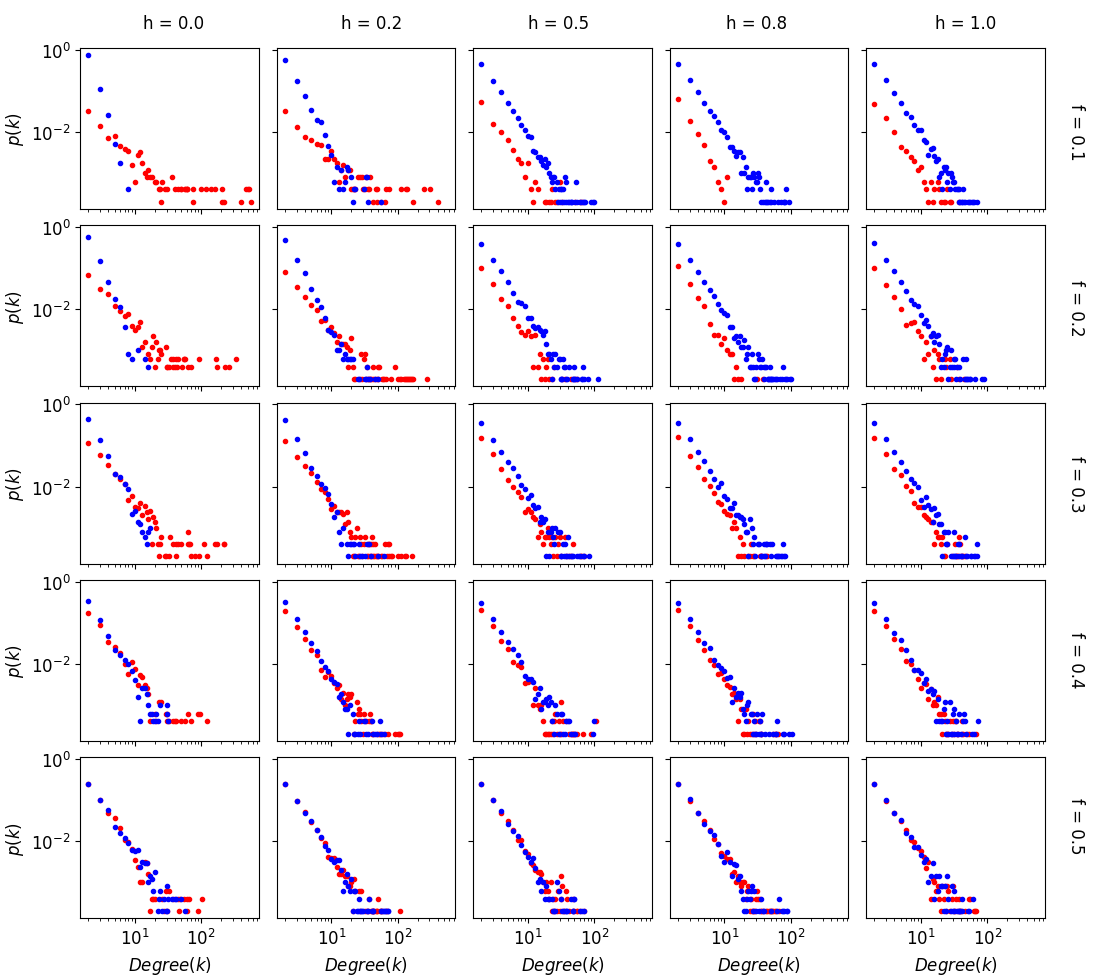
\includegraphics[width=1.0\textwidth]{images/dd_static.png}
	\caption{Degree distribution for static networks. The minority fractions are provided at the right-side of each row while the homophily is stated at the top of each column. Degree distribution for the majority and minority nodes are visualized using blue and red plot points respectively.}
	\label{dd_static_fig}
\end{figure}

Figure \ref{dd_static_fig} shows the plot for degree distribution of our generated synthetic networks. At the bottom row where both group sizes are same, the distribution is similar for all homophily values. As we go upwards towards networks with smaller minority group size, we see the disparity in distribution grow. Minority nodes are at an advantage in the heterophilic regime since they garner a lot of attention from the majority group. This changes as the homophily value increases putting majorities in favour as they prefer nodes from their own larger group. In a completely homophilic network, there exists in-group competition which decreases the difference in degree distribution values among groups.

\subsubsection{Degree Growth}

\begin{figure}[h!]
	\centering
	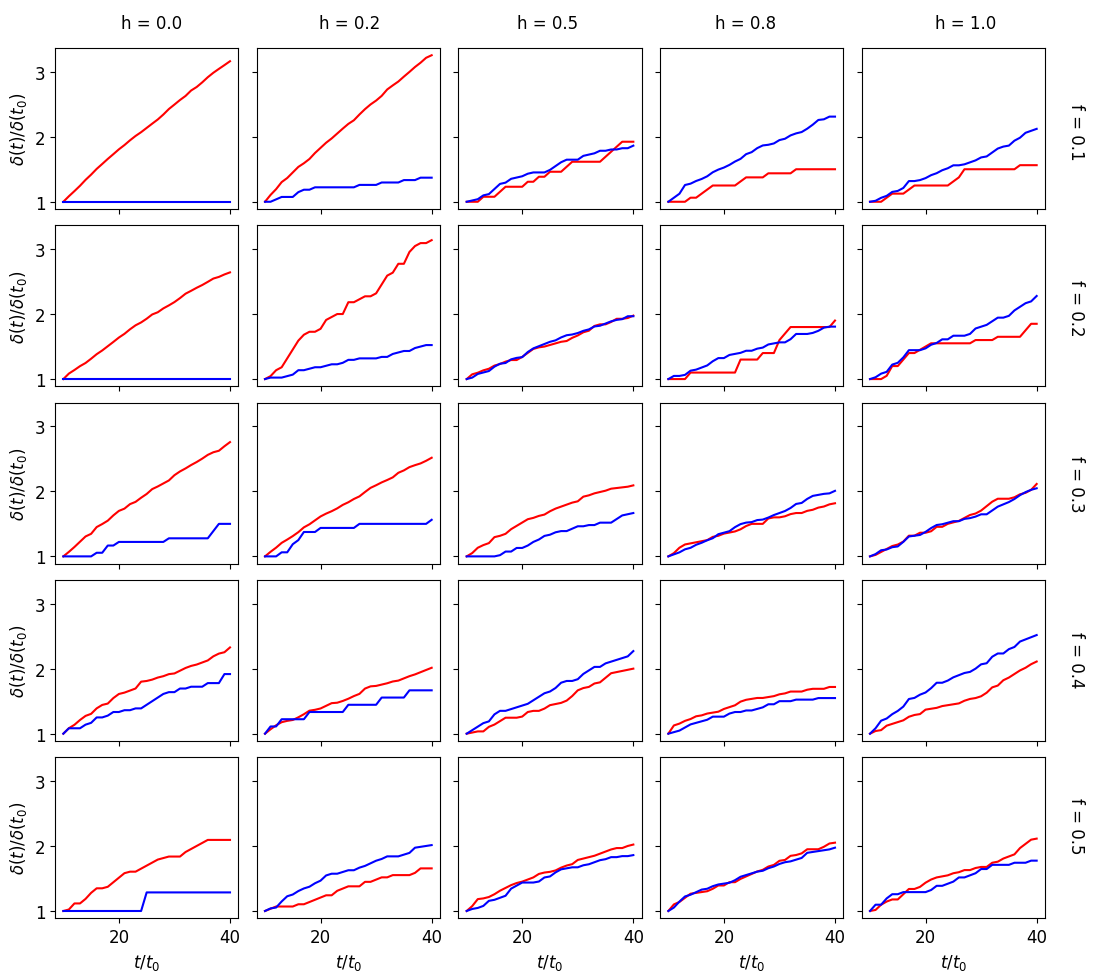
\includegraphics[width=1.0\textwidth]{images/dg_static.png}
	\caption{Degree growth for static networks. The minority fractions are provided at the right-side of each row while the homophily is stated at the top of each column. Degree growth for minority and majority node is visualized using the red and the blue color plot lines respectively.}
	\label{dg_static_fig}
\end{figure}

Figure \ref{dg_static_fig} shows how the degree of a majority and a minority node grows over time in the network generation process. We have realized before in our analysis of degree distribution, when the minority group size is small they tend to have higher degrees in heterophilic regime. In the homophilic regime, the majority groups have a slight advantage but due to competition amongst themselves this growth factor is small. We see in our plot however that when both group sizes are same, the minority has a higher growth over majority for $h=1.0$ and also the majority has a higher growth over minority at $h=0.8$. This is probably due to the choice of the nodes which contribute to the growth plot. We conducted similar network generation experiments for higher iteration values($t=5000$) and there we did not perceive this effect. We choose to keep these results though since these are the same networks we use in our later experiments. 

\subsubsection{Fraction of total degree held by minorities}

\begin{figure}[h!]
	\centering
	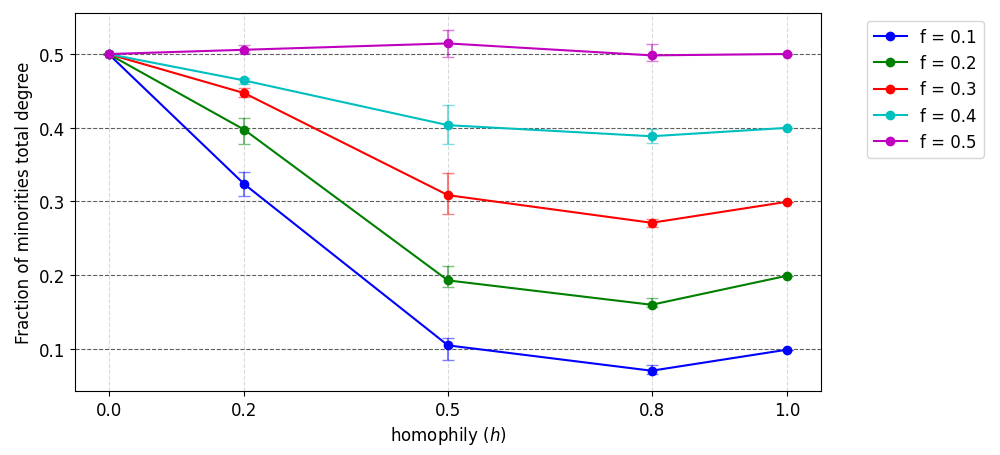
\includegraphics[width=0.8\textwidth]{images/mf_static.png}
	\caption{Fraction of total degree held by minority nodes in static networks at different minority fractions and different homophily values.}
	\label{mf_static_fig}
\end{figure}

Figure \ref{mf_static_fig} shows the fraction of total degrees held by the minority nodes in the network. In the heterophilic regime, the minority nodes hold a higher degree due to being favored by the majority nodes (which causes the \textit{``majority illusion''} problem). At $h=0.5$, where homophily doesn't play a role the degree fraction is nearly the same as minority group size. As we move towards the homophilic regime, the majority nodes do hold greater degree share at $h=0.8$ but this equalizes again as we near the complete homophily stage where the in-group support keeps both groups at appropriate degree share. 

\subsubsection{Top D\% degree rank}

\begin{figure}[h!]
	\centering
	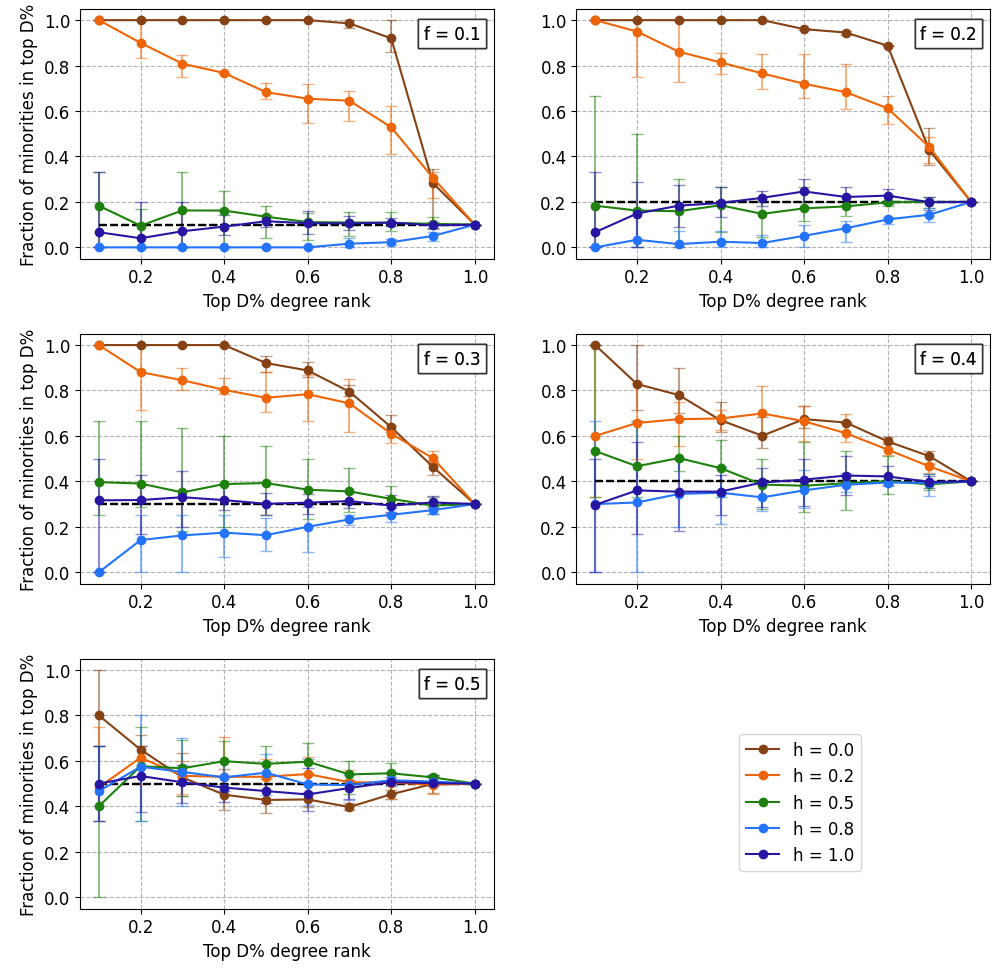
\includegraphics[width=1.0\textwidth]{images/top_static.png}
	\caption{The fraction of minority nodes found in top D\% nodes ranked according to degree in static networks. A black dotted line at each plot shows the actual fraction of minority nodes in the network.}
	\label{top_static_fig}
\end{figure}

Figure \ref{top_static_fig} shows the fraction of minority nodes which are present in the top D\% of node rankings (ranked according to degree). In heterophilic regime, the minority is highly over-represented than its group size, when the minority group size is small. This effect can be seen to reduce as the minority group size increases and the ranking at each percentage is closer to the original group size. At an equal group size, we can see that the degree rankings at each percentage adheres to the original group size.

\subsubsection{Disparate Visibility}
\label{static_dv}

\begin{figure}[h!]
	\centering
	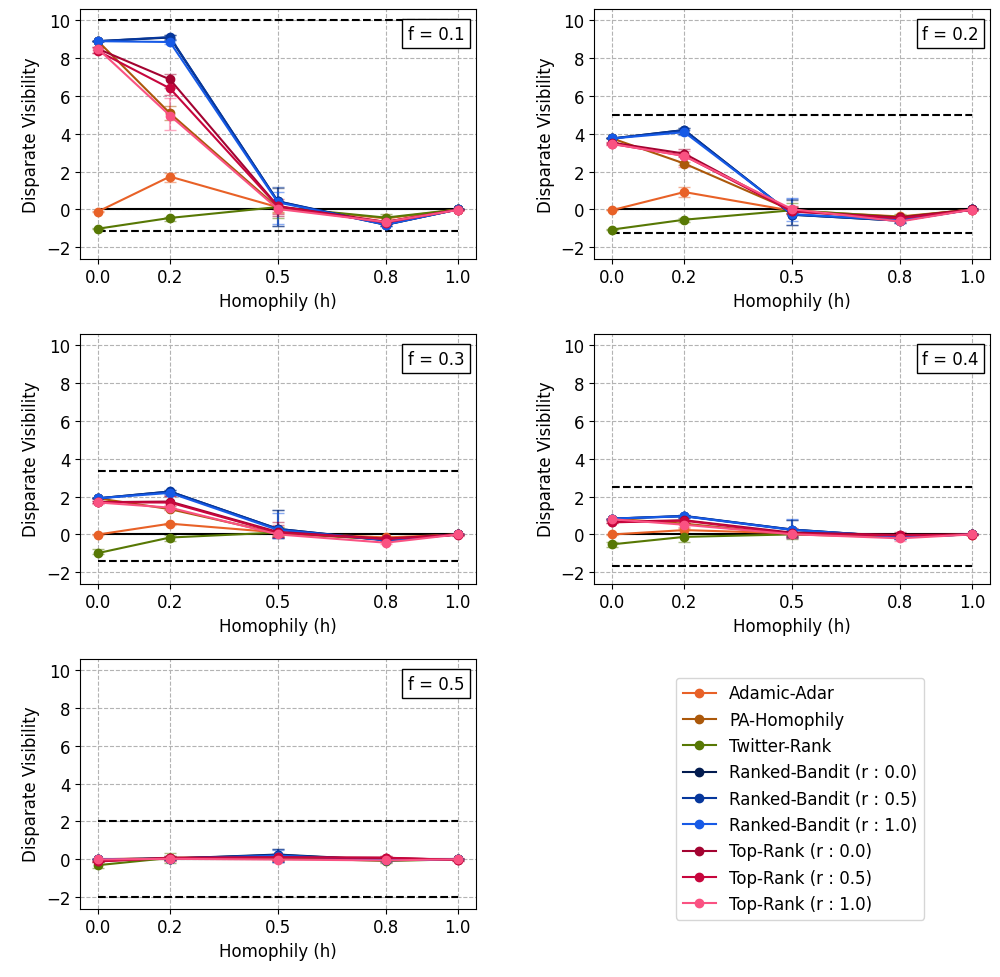
\includegraphics[width=1.0\textwidth]{images/dv_static.png}
	\caption{Disparate Visibility measure for static networks of different minority group sizes. The black line at each plot shows the equal visibility point and the black dotted lines represent the upper and lower limit for the disparate visibility measure.}
	\label{dv_static_fig}
\end{figure}

Figure \ref{dv_static_fig} shows the disparate visibility measure for the various recommendation methods. In the heterophilic regime we can see that minority nodes gain much higher visibility in recommendations for the \textbf{reinforcement methods} and \textbf{PA-Homophily} method. This we can expect as in the heterophilic regime the minorities are highly over-represented since they are likely to connect with the large number of majorities. As the minority fraction increases, this effect is seen to reduce. In the homophilic regime, although we see slight visibility gain for majority nodes at $h=0.8$ this is not that significant. The values lie quite close to equal visibility in recommendations at the homophilic regime.

For the \textbf{Adamic-Adar} and \textbf{Twitter-Rank} methods we observe a close stable measure with almost equal visibility for both groups at all homophily cases. 

For Adamic-Adar at $h=0$ we observe that the disparate visibility is always 0. This happens because in the case of complete heterophily, for Adamic-Adar, minority nodes are always suggested minority nodes and majority nodes are always suggested majority nodes. This happens owing to how the Adamic-Adar method works internally. To elaborate our point, we can consider the bipartite graph $G_t$ at $h=0$ as input to our recommender $R$ driven by Adamic-Adar. We know that Adamic-Adar suggests nodes based on common neighbours. Two minority nodes in $G_t$ would only have majority nodes in common at $h=0$ and thus a minority node would only be recommended to minorities. This same logic also holds in the case of a majority node recommendations. Thus, the disparate visibility is always at 0 in the case of complete heterophily for Adamic-Adar.

In the case of Twitter-Rank also we notice balanced visibility for both groups. While for Adamic-Adar we see from the plots that although there is equal visibility at $h=0$, the visibility for minorities is quite high at $h=0.2$. For Twitter-Rank however we can see that the visibility measure is quite near to the equal visibility line at all homophilies. 

\subsection{Summarized Findings}

We list down our observations from the experiments on Static Networks below.

\begin{enumerate}
	\item In the heterophilic regime, minority group nodes are at an advantage. In the homophilic regime, majority group nodes do tend to gain some advantage, but due to fierce competition amongst themselves this is very slight.
	
	\item As the minority group size increases and it gets closer to the equal group-size ($f=0.5$), the minorities start losing advantage over the majority in heterophilic regime. This phenomenon is also true for the majorities in the homophilic regime.
	
	\item The bias in recommendations received with different recommendation systems are highest in the case of \textbf{reinforcement methods} and \textbf{PA-Homophily} at the heterophilic regime. In the homophilic regime the visibility is close to equal for both groups. \textbf{Twitter-Rank} provides best equality in visibility for both groups in recommendations, also closely followed by \textbf{Adamic-Adar}.
	
\end{enumerate}

\section{Growing Networks}
\label{growing_networks}
In this section we propagate growth of synthetic networks, in which the growth is influenced by the use of different recommender systems $R$. In the experimental setup sub-section we lay down the detailed algorithm which we use for growing these networks. In the results sub-section we look in detail at the different properties of these recommendation influenced networks.

\subsection{Experimental Setup}
We generate our network by using algorithm \ref{growing_network_model}. We take influence from the \textit{recommendation algorithm model} by Stoica et. al. \cite{stoica2018algorithmic} while developing our growth algorithm. The key difference between the two approaches is the usage of a generic recommendation engine $R$ in our case and the usage of the karimi model \cite{karimi2018homophily} to make edge-formation decisions. 

\begin{algorithm}
	\SetAlgoLined
	\DontPrintSemicolon
	\SetKwInOut{Input}{input}\SetKwInOut{Output}{output}
	\Input{Total iterations : $t$\\Symmetric homophily value : $h$\\Probability of node being marked as minority node: $f$\\Recommender Engine : $R$\\Organic Growth Probability : $\alpha$\\Randomness : $\mu$\\Number of recommendations : $k$\\}
	\Output{Network : $G_{t}(V_{t},E_{t})$}
	\BlankLine
	With probability $f$ mark node $v_{0}$ as minority, else mark as majority.\;
	$V_{0} = \{v_{0}\}$\;
	\For{$i \leftarrow 1$ \KwTo $t$}{
		With $\alpha$ probability, choose $growth\_type$ as $organic$, else choose $algorithmic$.\;
		\uIf{$growth\_type$ is $organic$}{
			$V_{i} = V_{i-1} \cup \{v_{i}\}$\;
			With probability $f$ mark node $v_{i}$ as minority, else mark as majority.\;
			With probability $\mu$ choose $random\_connect$ as true, else choose false.\;
			\eIf{$random\_connect$ is true}{
				Choose node $u_{i}$ from $V_{i-1}$ at random.\;
			}{
				\ForEach{vertex $u \in V_{i-1}$}{
					$\Pi_{u} = (\delta(u) \times h_{uv_{i}}) / \sum_{w \in V_{i-1}}^{} (\delta(w) \times h_{wv_{i}}) $\; 
				}
				Choose $u_{i}$ based on probability $\Pi_{u \in V_{i-1}}$\;
			}
		}
		\ElseIf{$growth\_type$ is $algorithmic$}{
			$V_{i} = V_{i-1}$\;
			Choose $v_{i}$ from $V_{i}$ at random.\;
			Get recommendation list $L_{v_{i}} (|L_{v_{i}}|=k)$ for $v_{i}$ from recommender engine $R$.\;
			\ForEach{vertex $u \in L_{v_{i}}$}{
				$\Pi_{u} = (\delta(u) \times h_{uv_{i}}) / \sum_{w \in L_{v_{i}}}^{} (\delta(w) \times h_{wv_{i}}) $\; 
			}
			Choose $u_{i}$ based on probability $\Pi_{u \in L_{v_{i}}}$.\;
		}
		\eIf{$u_{i}$}{
			$E_{i} = E_{i-1} \cup \{(u_{i},v_{i})\}$\;
		}{
			$E_{i} = E_{i-1}$\;	
		}
	}
	\caption{Growing network model}\label{growing_network_model}
\end{algorithm}

In table \ref{table_growth_model} we list down the various tuneable and static parameters in our experimental setup for algorithm \ref{growing_network_model}. As the recommendation engine $R$, we use the following methods: PA-Homophily, Adamic-Adar, Twitter-Rank, Ranked-Bandit, Top-Rank (which we have discussed in detail in chapter \ref{recommender_methods}). The additional parameters used by the reinforcement methods are the same as listed in table \ref{table_recommendation}.

\begin{table}[h]
	\centering
	\begin{tabular}{ |c|c| }
		\hline
		\textbf{Parameter} & \textbf{Value} \\
		\hline
		Total iterations ($t$) & 10000 \\
		Randomness ($\mu$) & 0.1 \\
		Organic growth probability ($\alpha$) & 0.1 \\
		Symmetric homophily value ($h$) & [0.0, 0.2, 0.5, 0.8, 1.0] \\
		Probability of minority node ($f$) & [0.1, 0.2, 0.3, 0.4, 0.5] \\
		Number of recommendations ($k$) & 5 \\
		Recommender training iterations ($T$) & 10000 \\
		Ranking factor ($r$) & [0.0, 0.5, 1.0] \\
		\hline
	\end{tabular}
	\caption{Parameters for generation of synthetic networks as outlined by algorithm \ref{growing_network_model}}
	\label{table_growth_model}
\end{table}

What we can observe from our algorithm given the experimental setup is that the synthetic networks which we receive as output would be having more number of edges than the previous synthetic networks used in section \ref{static_networks} owing to \textit{algorithmic growth}. The total number of iterations for the generation of $G_{t}$ is $t=10000$. Given the organic growth probability $\alpha=0.1$, we expect the total number of nodes $|V_{t}| \simeq 1000$. Since the number of edges are quite high, owing to \textit{algorithmic growth}, the average degree of nodes also increases, which can be seen very specifically in some plots (specially that of \textit{Adamic-Adar}). Also another notable difference with the networks generated in section \ref{static_networks} is that $h=0$ may not mean a completely bipartite graph in the case of \textit{growing networks} since there is a randomness factor $(\mu)$ at play here. Also by similar logic, for a value of $h=1$ the synthetic network might not be completely disjoint. How all these factors come together and influence the network growth we will be seeing in the next few sections.

Now that we have detailed the experimental setup, we generate synthetic networks by tuning the different parameters in table \ref{table_growth_model}, having 5 simulations for each variation. In the subsequent sections we list the various results for our experiments and also our analysis for them. 

\subsection{Experimental Results : PA-Homophily}

\begin{figure}[h!]
	\centering
	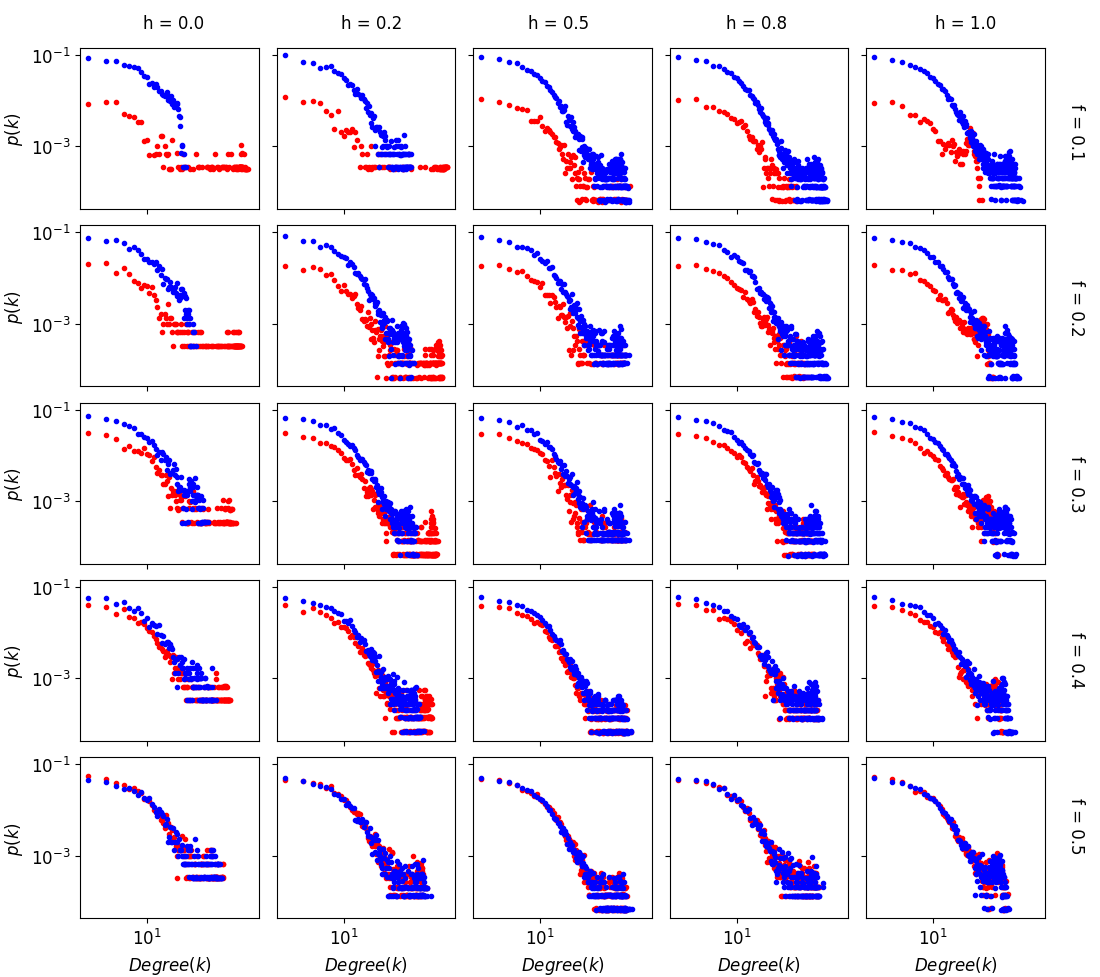
\includegraphics[width=1.0\textwidth]{images/dd_growth_pa.png}
	\caption{Degree distribution for growing networks with \textbf{PA-Homophily}. The minority fractions are provided at the right-side of each row and the homophily values are specified at the top of each column. Degree distribution for the majority and minority nodes are visualized using blue and red plot points respectively.}
	\label{dd_growth_pa_fig}
\end{figure}

\begin{figure}[h!]
	\centering
	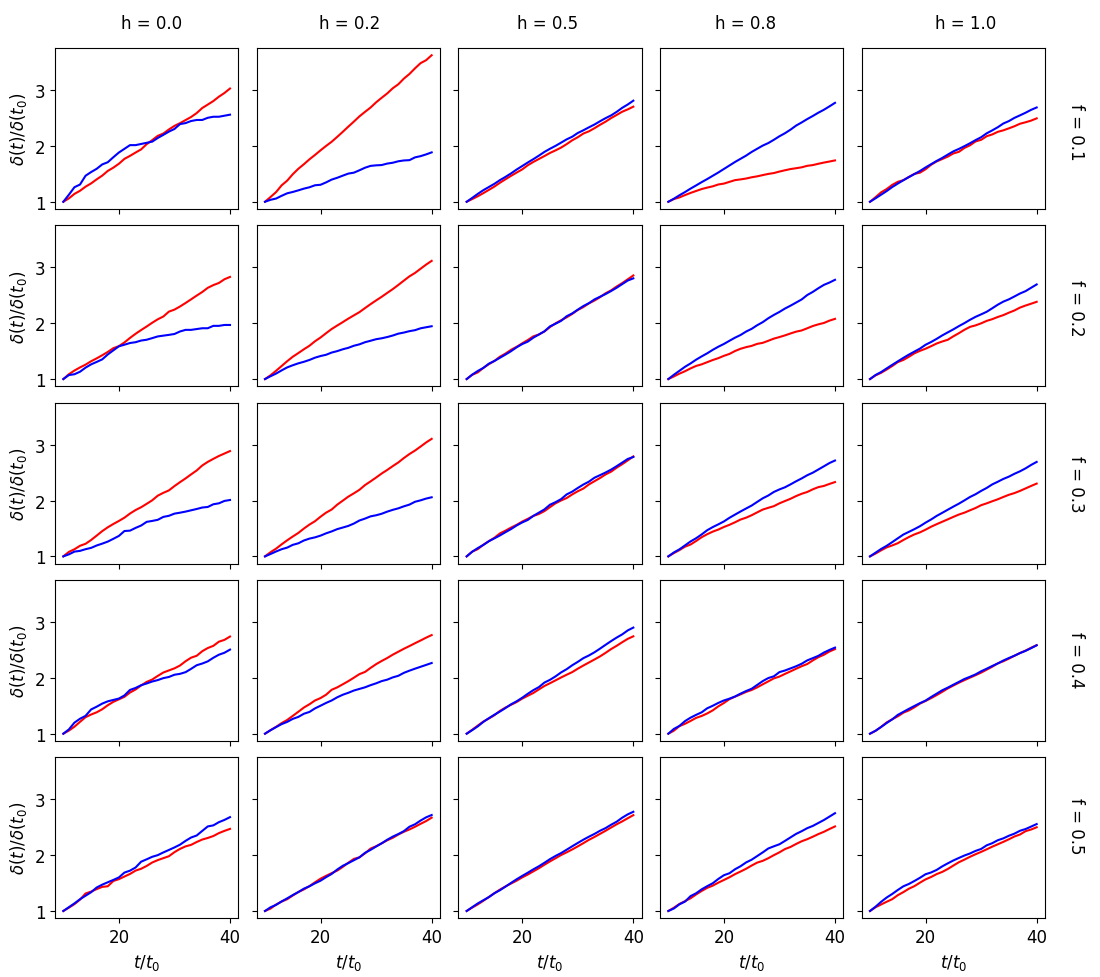
\includegraphics[width=1.0\textwidth]{images/dg_growth_pa.png}
	\caption{Degree growth for growing networks with \textbf{PA-Homophily}. The minority fractions are provided at the right-side of each row and the homophily values are specified at the top of each column. Degree growth for minority and majority node is visualized using red and blue color plot lines respectively.}
	\label{dg_growth_pa_fig}
\end{figure}

\begin{SCfigure}[1][h!]
	\centering
	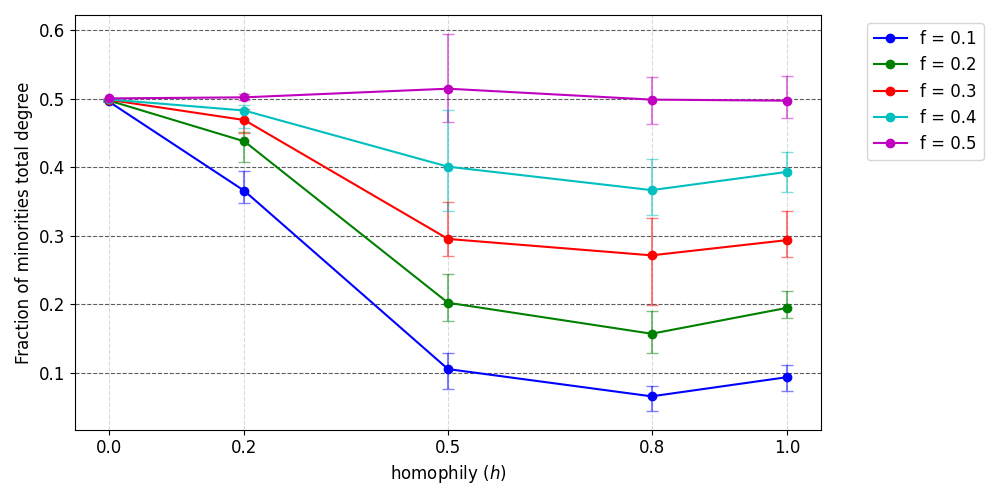
\includegraphics[trim=0 5 0 10, clip, width=0.75\textwidth]{images/mf_growth_pa.png}
	\caption{The fraction of total degree held by minority nodes for growing networks with \textbf{PA-Homophily}.}
	\label{mf_growth_pa_fig}
\end{SCfigure}

\begin{figure}[h!]
	\centering
	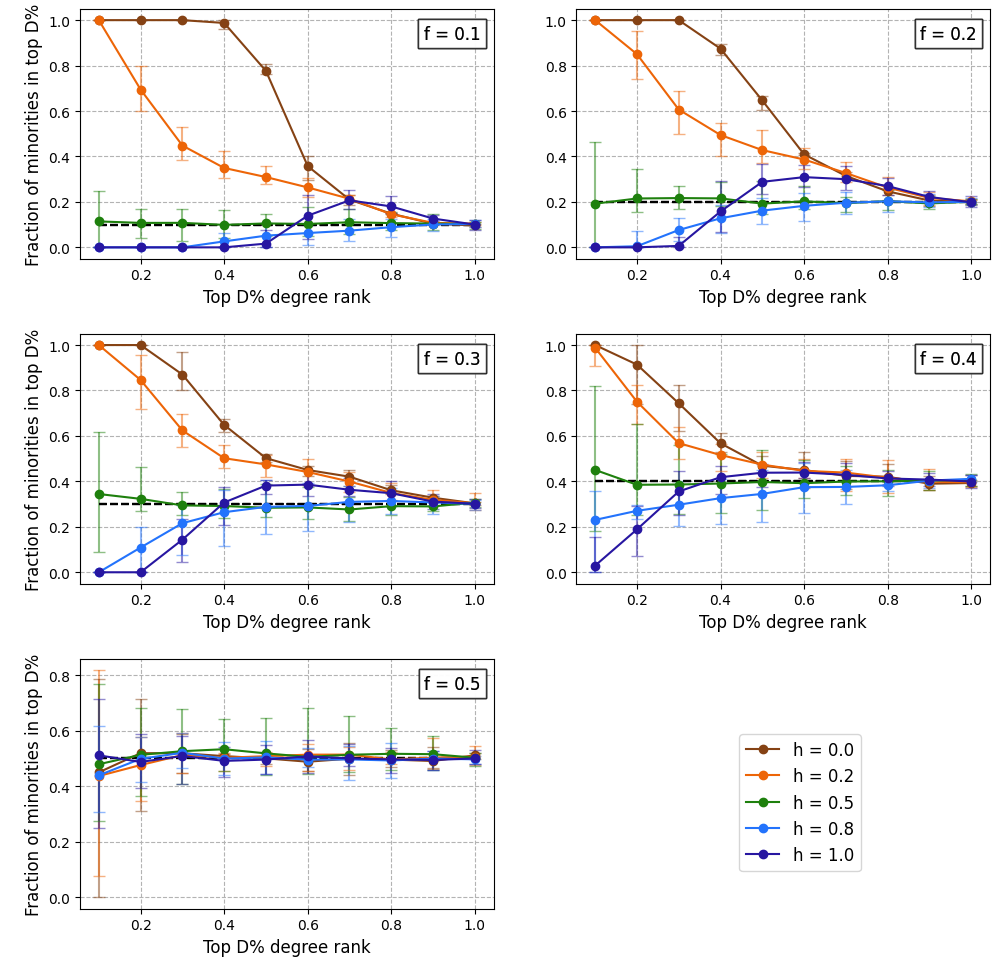
\includegraphics[trim=0 10 0 5, clip, width=1.0\textwidth]{images/top_growth_pa.png}
	\caption{The fraction of minority nodes found in top D\% nodes ranked according to degree in growing networks with \textbf{PA-Homophily}. A black dotted line at each plot shows the actual fraction of minority nodes in the network.}
	\label{top_growth_pa_fig}
\end{figure}

In the case of \textit{PA-Homophily}, the recommender method calculates probability of candidate nodes to be chosen for connection with seeking node by considering parameters like degree of the candidate nodes and homophily between the candidate and the seeking node.

In the \textbf{heterophilic} regime, we can see that the minority nodes have a clear edge over majority nodes and this is higher in case of lower minority group sizes. The large number of majority nodes in this regime choose to give attention to the fewer minority nodes which lead to these minorities ultimately holding higher degrees. This can be seen from the degree distribution plot (figure \ref{dd_growth_pa_fig}).

From the degree growth plot (\ref{dg_growth_pa_fig}) we can see that minorities would have higher degree growth than majorities due to this attention from majorities. They also hold very high amount of the total degree in the networks as can be seen in figure \ref{mf_growth_pa_fig}. This clearly shows that the minorities are having a high over-representation in this regime. Ranking the nodes according to their degrees confirms this for us as we can see in figure \ref{top_growth_pa_fig} that the top rank holders are mostly minority nodes. The recommendation lists for minorities and majorities have nodes from the other groups highly and thus driven by the algorithmic growth this gives us a network similar to what we get from the models generated by algorithm \ref{algo_karimi_model} in the case of \textit{static networks}.

In the \textbf{homophilic} regime, from the degree distribution plot (figure \ref{dd_growth_pa_fig}) we see that majorities tend to hold higher degrees than minorities which is expected since the groups tends tend to connect amongst themselves and the majorities are larger in number.

We also see that the minority nodes are recommended a lot more majority nodes in their recommendation lists, specially when the minority size is very low and homophily is $h=0.8$. At $h=0.8$, the majority has higher growth but the difference with growth of minorities is not very high.

At complete homophily only in-group support is present so then the reversed effect of $h=0$ can be seen for lower minority fractions. Looking at the plot in figure \ref{mf_growth_pa_fig} we can see that the minorities share of total degrees is only slightly lower than its group size at $h=0.8$. Ranking these nodes according to degree as done in figure \ref{top_growth_pa_fig} shows that minorities are underrepresented. At $h=1$ we see that the minorities tend to be over-represented at about the $D=40\%$ mark. We saw this effect slightly before in our pre-generated synthetic networks in figure \ref{top_static_fig}. We have confirmed that this effect is not seen for networks with about 5000 nodes and we believe that this is only seen due to the less number of nodes we use in our networks. Also, the randomness factor ($\mu$) adds an extra exaggeration to this effect which might be another factor to cause this kind of over-representation for our plots in the \textit{growing networks} perspective.

\subsection{Experimental Results : Adamic-Adar}

In the case of \textit{Adamic-Adar}, the growth is completely based on the network structure that develops over time. The recommendation system is agnostic of the type of nodes it is dealing with when recommending and is solely dependent on the neighbours of the seeker and candidate nodes used to calculate the Adamic-Adar index. 

\begin{figure}[h!]
	\centering
	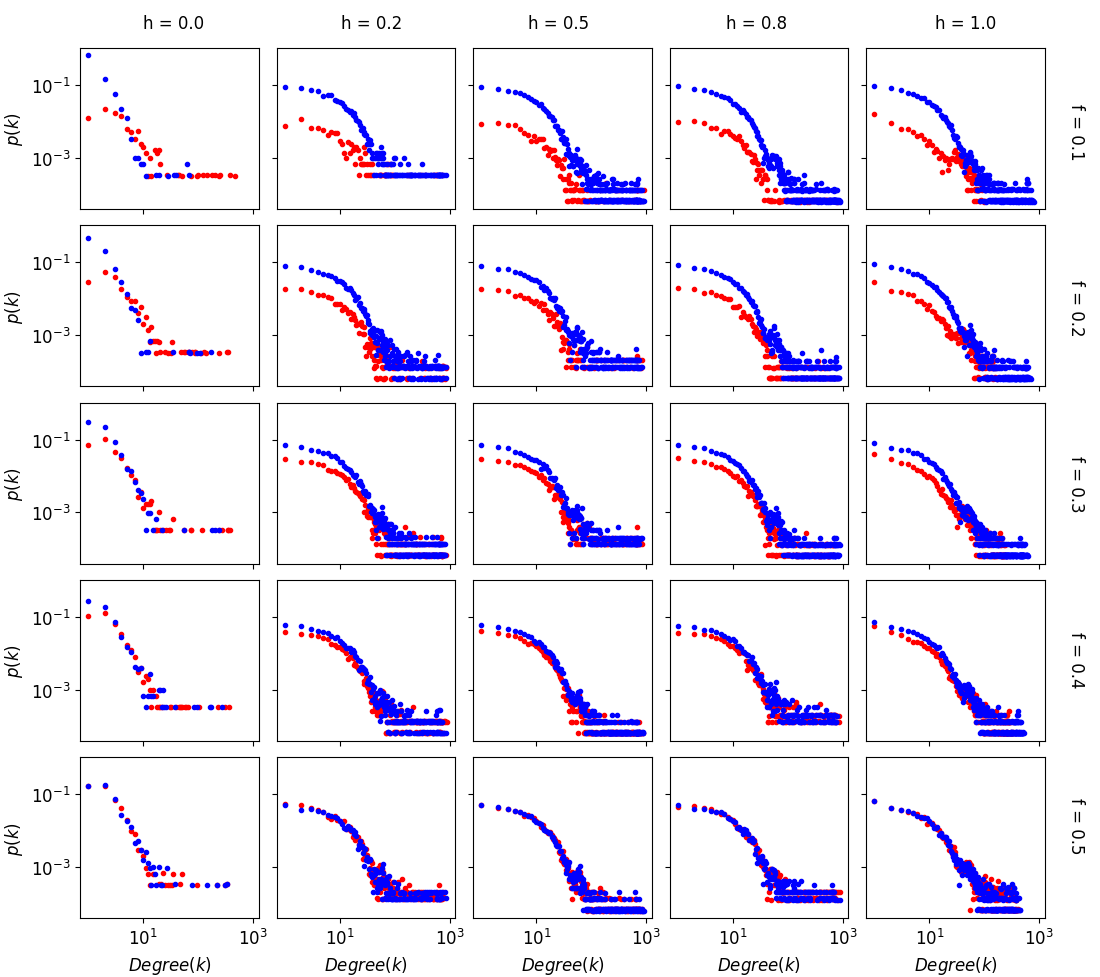
\includegraphics[width=1.0\textwidth]{images/dd_growth_aa.png}
	\caption{Degree distribution for growing networks with \textbf{Adamic-Adar}. The minority fractions are provided at the right-side of each row and the homophily values are specified at the top of each column.  Degree distribution for the majority and minority nodes are visualized using blue and red plot points respectively.}
	\label{dd_growth_aa_fig}
\end{figure}

\begin{figure}[h!]
	\centering
	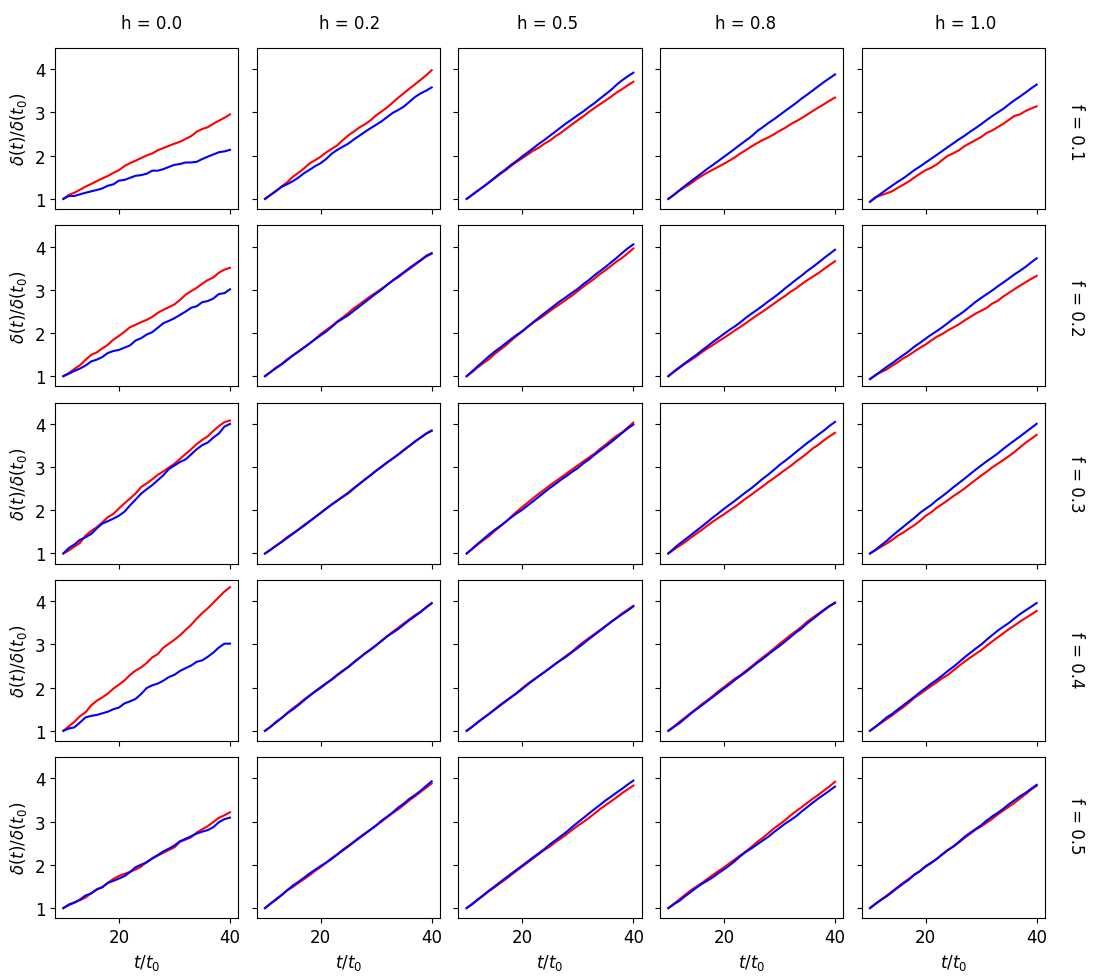
\includegraphics[width=1.0\textwidth]{images/dg_growth_aa.png}
	\caption{Degree growth for growing networks with \textbf{Adamic-Adar}. The minority fractions are provided at the right-side of each row and the homophily values are specified at the top of each column. Degree growth for minority and majority node is visualized using red and blue color plot lines respectively.}
	\label{dg_growth_aa_fig}
\end{figure}

\begin{SCfigure}[1][h!]
	\centering
	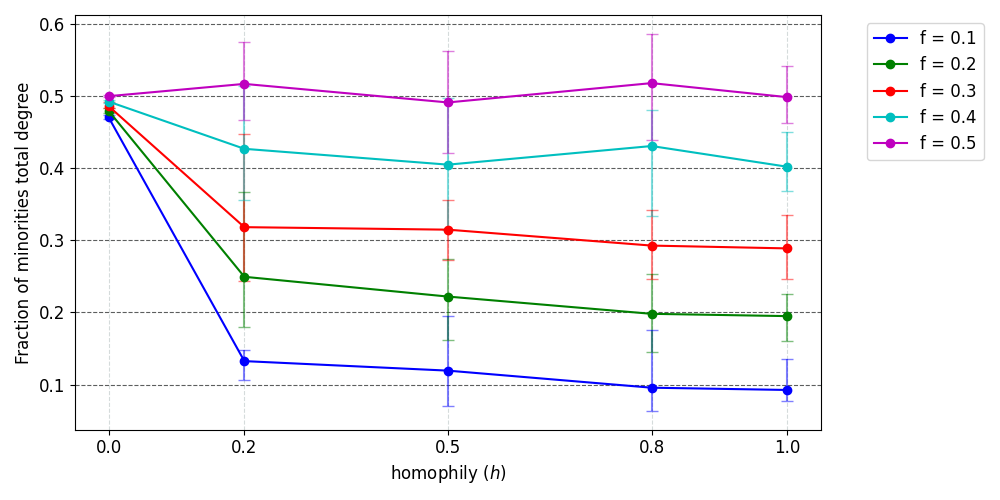
\includegraphics[trim=0 5 0 10, clip, width=0.75\textwidth]{images/mf_growth_aa.png}
	\caption{The fraction of total degree held by minority nodes for growing networks with \textbf{Adamic-Adar}.}
	\label{mf_growth_aa_fig}
\end{SCfigure}

\begin{figure}[h!]
	\centering
	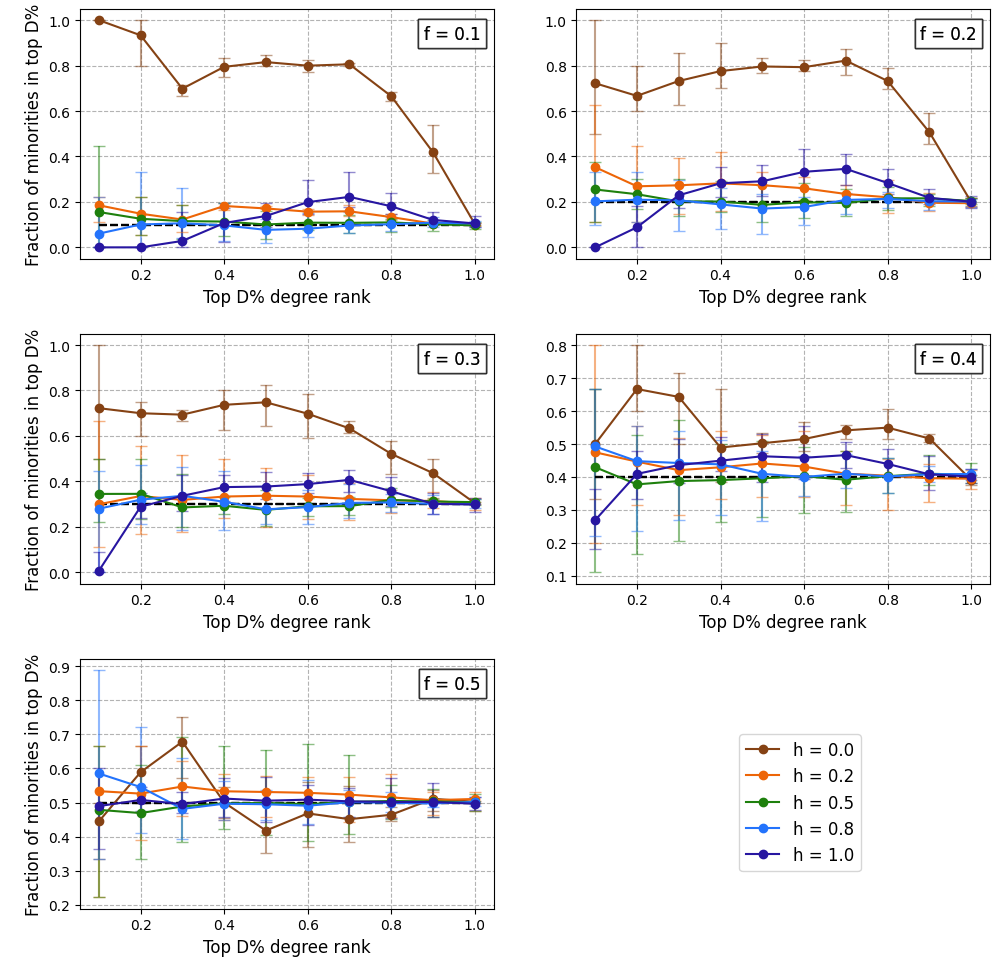
\includegraphics[trim=0 10 0 5, clip, width=1.0\textwidth]{images/top_growth_aa.png}
	\caption{The fraction of minority nodes found in top D\% nodes ranked according to degree in growing networks with \textbf{Adamic-Adar}. A black dotted line at each plot shows the actual fraction of minority nodes in the network.}
	\label{top_growth_aa_fig}
\end{figure}

Let us consider the \textbf{heterophilic} regime, where nodes prefer to get connected with nodes from the opposite group. In the extreme heterophilic case, nodes simply reject connection with nodes from the other group. If we consider homophily value of $h=0$, the nodes from same group which are suggested would be completely rejected for connections thus most of the recommendations would not result in any fruitful connections. However at $h=0.2$, even with weak probability they would connect which helps evolve the structure of the network unbiased. This difference between behavior at the two homophily values causes a stark difference in the degree distribution plot (figure \ref{dd_growth_aa_fig}) for Adamic-Adar. 

Also in the degree distribution plot (figure \ref{dd_growth_aa_fig}) we see that while at the extreme heterophily case ($h=0$), minority nodes do hold higher degrees in most cases, but with the change in minority group size there is not much change. It can be seen that the probability of having a lower degree minority node seems to be increasing with the increase in minority group size.

The degree growth plot (figure \ref{dg_growth_aa_fig}) shows that at $h=0$ homophily there is a slightly higher degree growth for the minorities which mostly happens due to the organic growth of the network. As the strict heterophily is relaxed and minorities start connecting with majorities even with weaker probabilities, we can see that both the minorities and majorities have high degree growth with time.

This can be further verified by checking the fraction of total degrees held by minority nodes (figure \ref{mf_growth_aa_fig}) where at $h=0.2$ we see that the minorities hold degree close to its original size. Also with the degree ranking plot (figure \ref{top_growth_aa_fig}) it is seen that the plot lines lie close to the fraction of minorities in the network at $h=0.2$ which signifies a balanced network. At $h=0$ we do see over-representation but that is only due to the strict heterophily measure and with even the slightest lax network would ease up towards the unbiased structure. 

In the \textbf{homophilic} regime, at $h=0.8$ there is high recommendation of majorities for both the minority and majority seeker nodes. The lesser the minority size the more majority nodes are recommended by the recommender. This is what aides the majorities to gain very high degrees compared to minorities in the case of $h=0.8$.

At $h=1$, majorities start getting recommended majorities and minorities start getting recommended minorities. This causes the minority nodes to also gain higher degrees like majorities and thus have similar distribution as can be seen in figure \ref{dd_growth_aa_fig}. Looking at the degree growth plot (figure \ref{dg_growth_aa_fig}) we see that both type of nodes have high degree growth with the majorities maybe slightly leading in the case of lower minority fractions. Since the degree of both type of nodes have similar growth we can also see that the fraction of total degrees held by both type of nodes is almost balanced according to the minority fraction of the network. This signifies that the minorities have almost the same representation as their group-size in degree ranking which can be seen in figure \ref{top_growth_aa_fig}.

The observation which we can draw from the Adamic-Adar recommendations is that the type of recommended nodes which the seeker nodes receive is almost similar at the extreme cases of homophily and heterophily. This harms in edge-connection in $h=0$ but helps in $h=1$. For the in-between cases there is always higher number of majority nodes recommended for both type of nodes which causes the visibility of the majorities to be at par with its group size.

\subsection{Experimental Results : Twitter-Rank}

\textbf{Twitter-Rank} bases ranking on the SALSA scoring mechanism. The nodes in hubs and authorities are formed by collecting nodes to form a ``circle of trust'' (hub side) and the nodes connecting  to the hubs (authorities side) which are then ranked according to the SALSA scores and provided as recommendations.

\begin{figure}[h!]
	\centering
	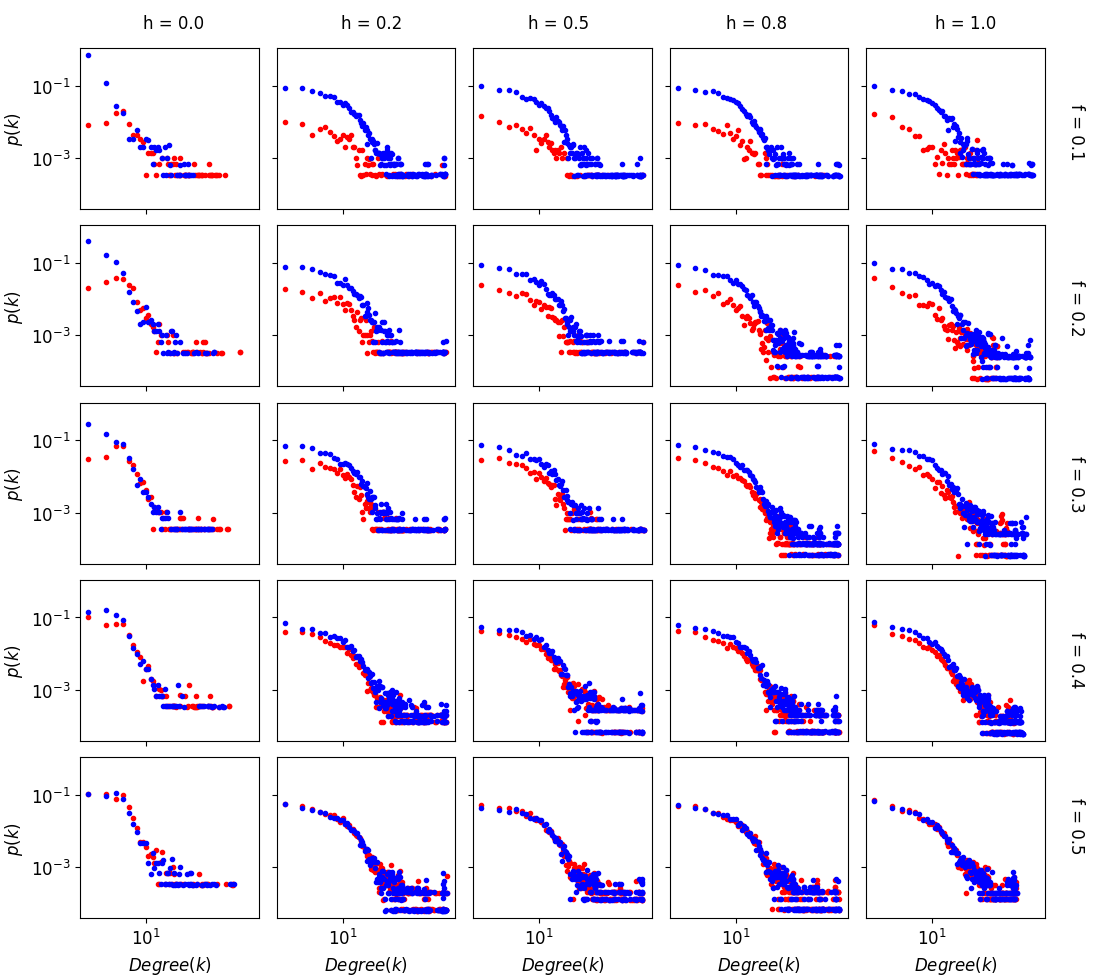
\includegraphics[width=1.0\textwidth]{images/dd_growth_tr.png}
	\caption{Degree distribution for growing networks with \textbf{Twitter-Rank}. The minority fractions are provided at the right-side of each row and the homophily values are specified at the top of each column. Degree distribution for the majority and minority nodes are visualized using blue and red plot points respectively.}
	\label{dd_growth_tr_fig}
\end{figure}

\begin{figure}[h!]
	\centering
	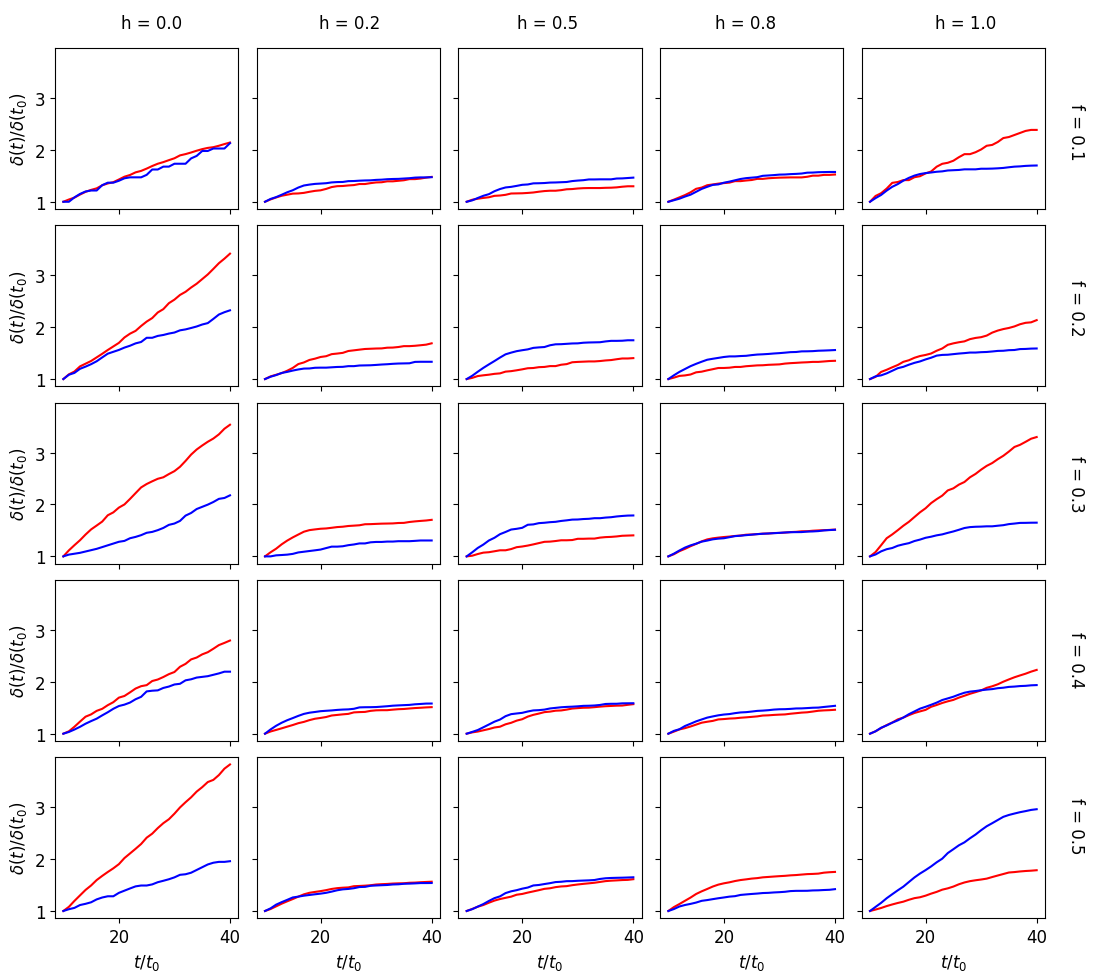
\includegraphics[width=1.0\textwidth]{images/dg_growth_tr.png}
	\caption{Degree growth for growing networks with \textbf{Twitter-Rank}. The minority fractions are provided at the right-side of each row and the homophily values are specified at the top of each column. Degree growth for minority and majority node is visualized using red and blue color plot lines respectively.}
	\label{dg_growth_tr_fig}
\end{figure}

\begin{SCfigure}[1][h!]
	\centering
	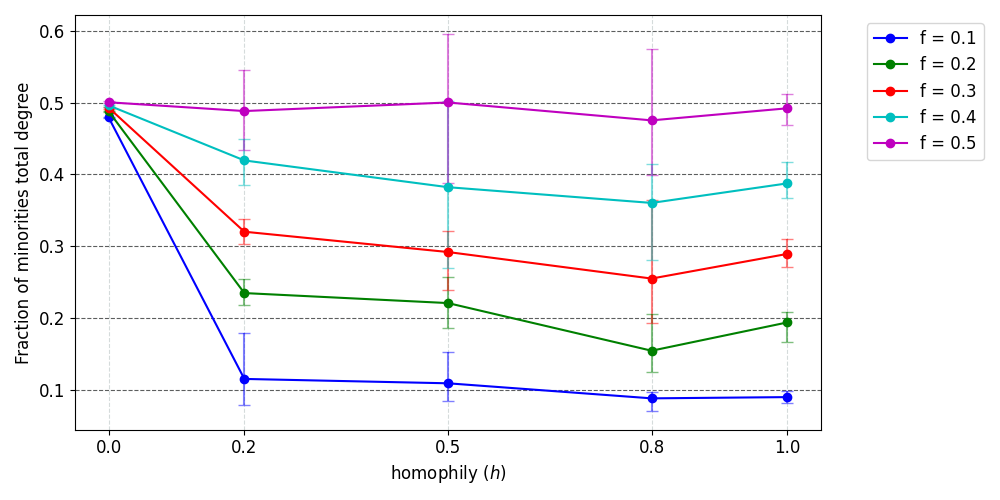
\includegraphics[trim=0 5 0 10, clip, width=0.75\textwidth]{images/mf_growth_tr.png}
	\caption{The fraction of total degree held by minority nodes for growing networks with \textbf{Twitter-Rank}.}
	\label{mf_growth_tr_fig}
\end{SCfigure}

\begin{figure}[h!]
	\centering
	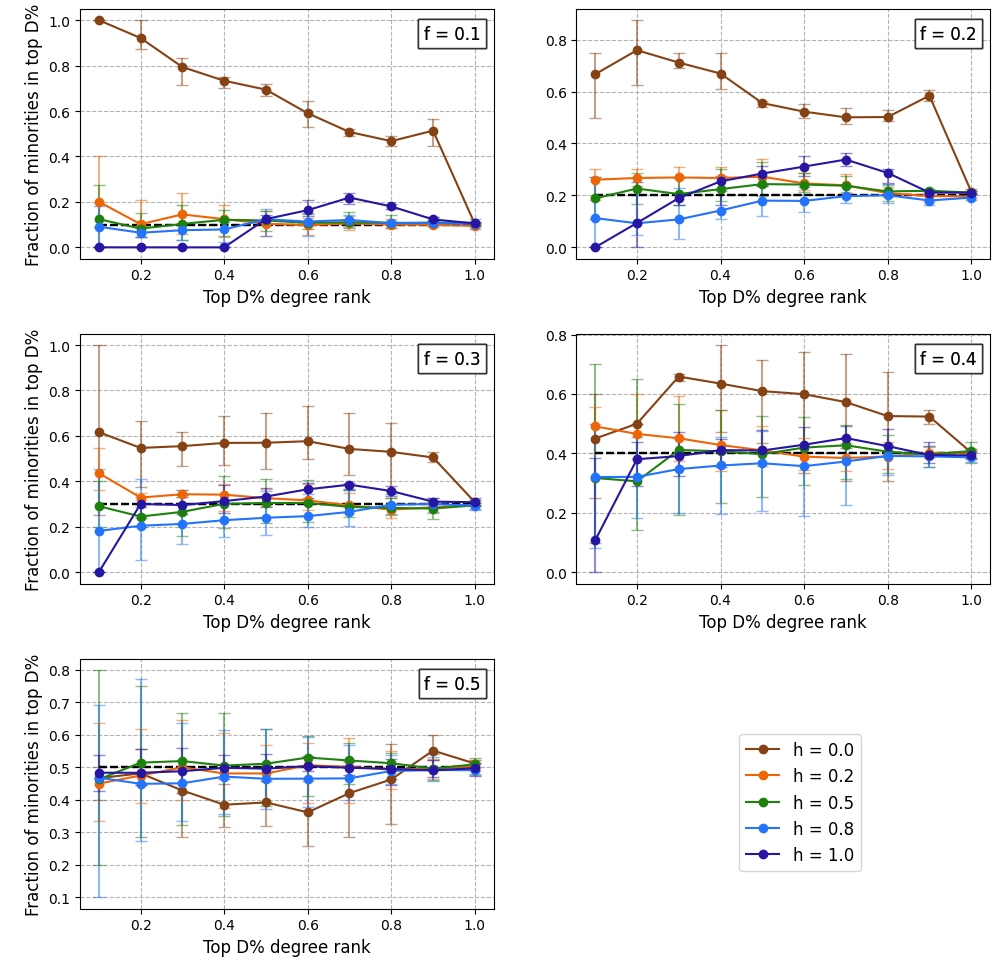
\includegraphics[trim=0 10 0 5, clip, width=1.0\textwidth]{images/top_growth_tr.png}
	\caption{The fraction of minority nodes found in top D\% nodes ranked according to degree in growing networks with \textbf{Twitter-Rank}. A black dotted line at each plot shows the actual fraction of minority nodes in the network.}
	\label{top_growth_tr_fig}
\end{figure}

First we would be discussing about behavior in the \textbf{heterophilic} regime. At $h=0$, majorities are recommended an incredibly high amount of majority nodes and minorities are recommended minority nodes (this increases with the group size). For a smaller minority group size at $h=0$, it can be seen that there is more majorities which are recommended for minorities but with time this also drops. This explains why at $h=0$, the nodes do not attain very high degrees as can be seen in the degree distribution plot (figure \ref{dd_growth_tr_fig}). The degree growth is quite high for minorities because over time they still receive a healthy number of majority node connections. The majorities however do not receive that much of minority connections so their degree growth is weak. 

At $h=0.2$, the distribution completely changes. At this phase majorities start getting recommended highly for both type of nodes. This provides the unbiased networks which have the fraction of total degrees close to that of the original group size (as seen in figure \ref{mf_growth_tr_fig}). We can see that although at the extreme case the minorities are overrepresented, as the homophily increases the network reaches a equal visibility relative to the group size. 

In the \textbf{homophilic} regime, at $h=0.8$ there is high number of majority node recommendations for both the majority and the minority nodes. Thus even in this case the degree is closer to the group size of the individual nodes. If we look at the fraction of total degrees held by minorities plot (figure \ref{mf_growth_tr_fig}) we see that minorities seem to be holding slightly lesser fraction of degree than its group size. This can be understood by the fact that while there is high number of recommendations of majorities for both groups, the count of majorities recommended for majorities is slightly less in the homophilic regime. At the complete homophily case since most of the network is possibly disconnected, nodes start getting recommendations from its own group as we had also observed previously in the \textit{PA-Homophily} case. 

An observation which we can make specifically from the degree growth plot (\ref{dg_growth_tr_fig}) is that in the range of $h=[0.2, 0.8]$ the degree growth is quite dampened. We believe that since in this method the user's `circle of trust' is formed based on the personalized PageRank mechanism the recommendation of nodes have a local effect, as in the recommended nodes belong in the locality of the seeker nodes. Thus, the degree of specific nodes might not grow as fast as seen in other methods. This also signifies that we do not reach very high degrees for nodes in this method as can be seen from the degree distribution plot (figure \ref{dd_growth_tr_fig}) compared to let's say \textit{Adamic-Adar} which causes the network nodes to have really high degrees. 

\subsection{Experimental Results : Ranked-Bandit}

In our experiments we modified the value of ranking factor ($r$) with values $\{0.0, 0.5, 1.0\}$ to influence the effect of ranking in the recommendation list $L_{v_{i}}$ for node $v_{i} \in V_{i}$. We however observed that this ranking factor $r$ provides very little difference to our plots. If we check the count of the recommendations which nodes get for different ranking values (check additional plots in appendices), we can see that at higher $r$ values there is a slight difference in the homophilic region for the number of nodes which are recommended for each type. This is however very minimal and we do not believe that it influences the choice of network nodes connection. In this section we display only the plots for the $r$ value of 1.0. The plots for other $r$ values can be found in the additional plots in appendices. 

\begin{figure}[h!]
	\centering
	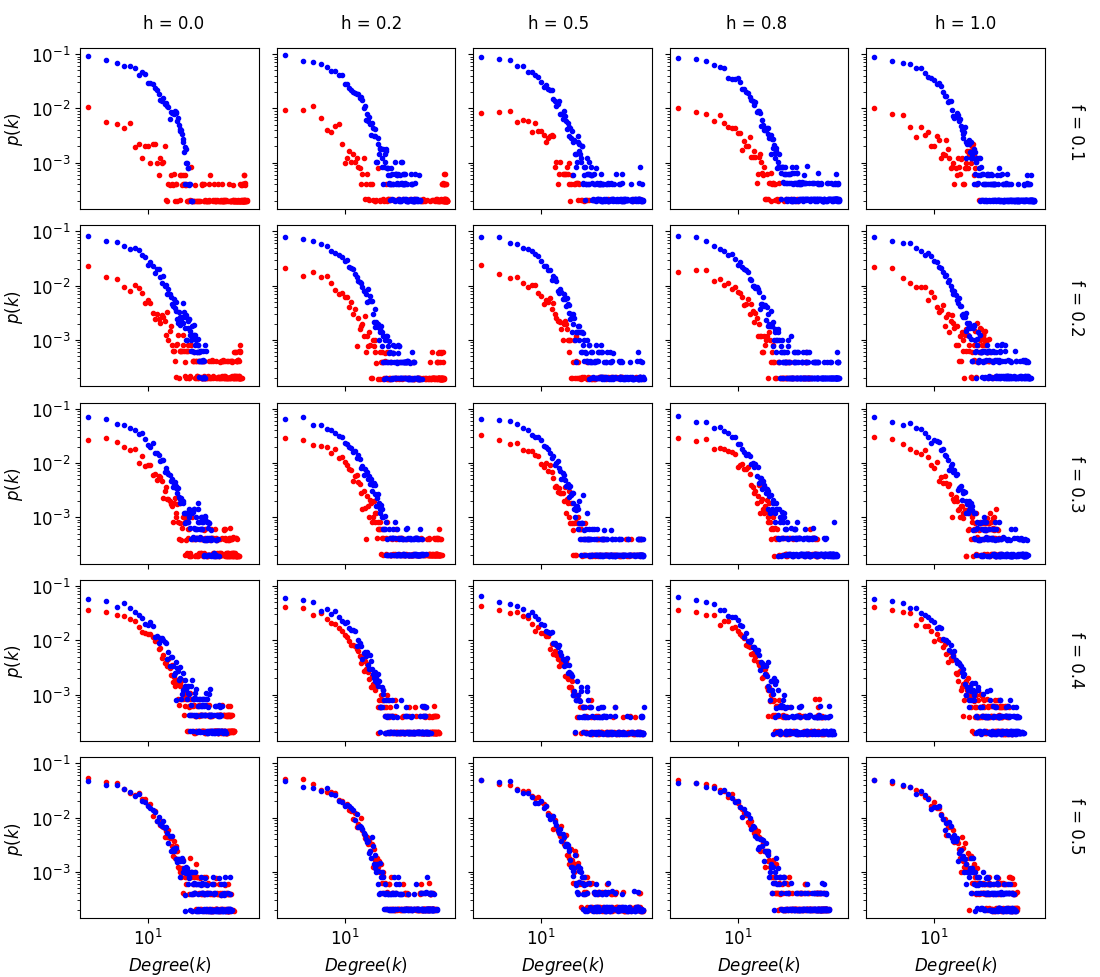
\includegraphics[width=1.0\textwidth]{images/dd_growth_rb10.png}
	\caption{Degree distribution for growing networks with \textbf{Ranked-Bandit ($r = 1.0$)}.The minority fractions are provided at the right-side of each row and the homophily values are specified at the top of each column. Degree distribution for the majority and minority nodes are visualized using blue and red plot points respectively.}
	\label{dd_growth_rb10_fig}
\end{figure}

\begin{figure}[h!]
	\centering
	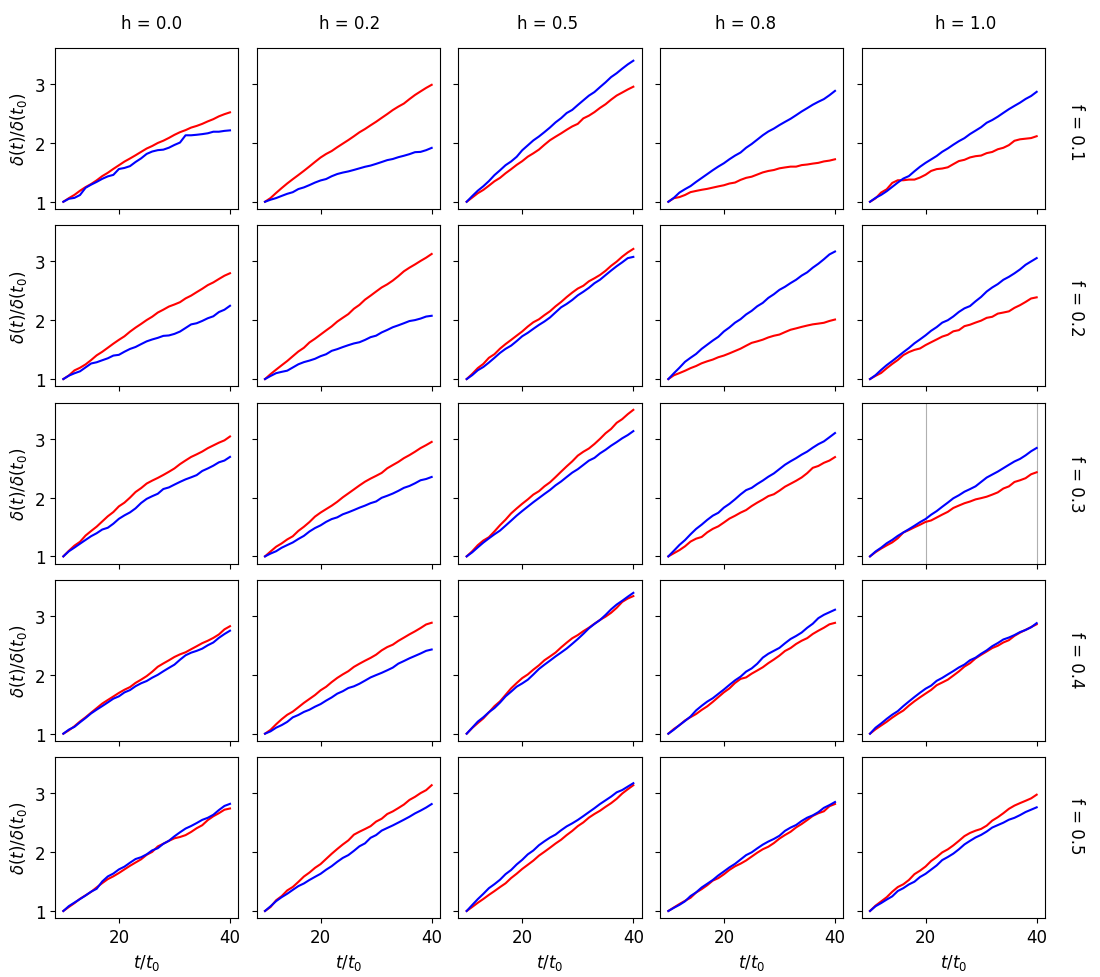
\includegraphics[width=1.0\textwidth]{images/dg_growth_rb10.png}
	\caption{Degree growth for growing networks with \textbf{Ranked-Bandit ($r = 1.0$)}. The minority fractions are provided at the right-side of each row and the homophily values are specified at the top of each column. Degree growth for minority and majority node is visualized using red and blue color plot lines respectively.}
	\label{dg_growth_rb10_fig}
\end{figure}

\begin{SCfigure}[1][h!]
	\centering
	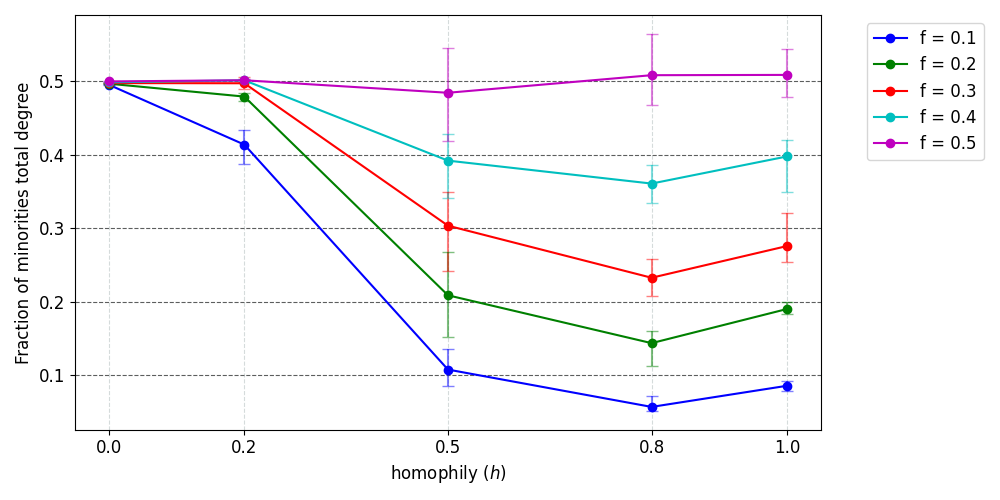
\includegraphics[trim=0 5 0 10, clip, width=0.75\textwidth]{images/mf_growth_rb10.png}
	\caption{The fraction of total degree held by minority nodes for growing networks with \textbf{Ranked-Bandit ($r = 1.0$)}.}
	\label{mf_growth_rb10_fig}
\end{SCfigure}

\begin{figure}[h!]
	\centering
	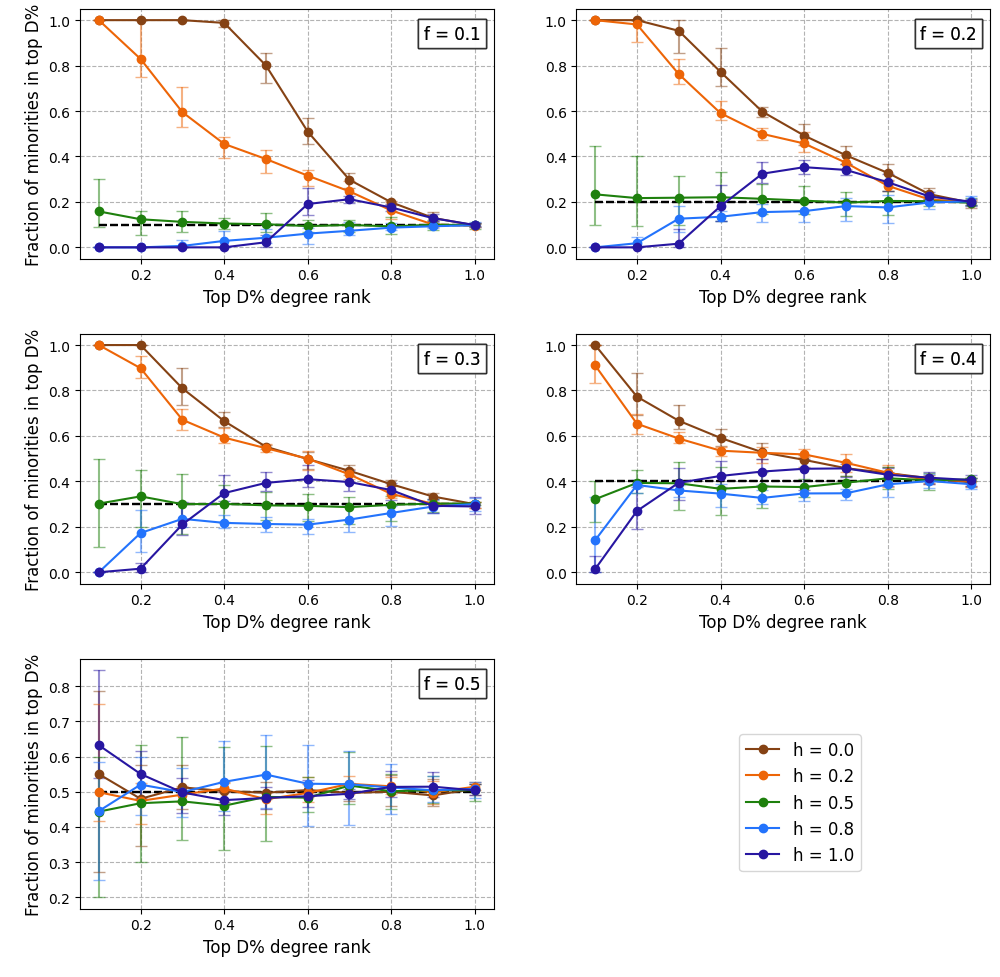
\includegraphics[trim=0 10 0 5, clip, width=1.0\textwidth]{images/top_growth_rb10.png}
	\caption{The fraction of minority nodes found in top D\% nodes ranked according to degree in growing networks with \textbf{Ranked-Bandit ($r = 1.0$)}. A black dotted line at each plot shows the actual fraction of minority nodes in the network.}
	\label{top_growth_rb10_fig}
\end{figure}

If we observe the degree distribution while using the \textbf{Ranked-Bandit} method in figure \ref{dd_growth_rb10_fig}, we can see that owing to the use of the click model (which in turn uses the Karimi model \cite{karimi2018homophily}) we see the patterns which could be observed in figure \ref{dd_growth_pa_fig} also observed here. In the heterophilic regime, minority nodes hold higher degrees than majority nodes and as we move towards the homophilic regime, this reverses. Also as we move down the figure towards increasing minority group sizes we can see that the degree distribution for both group of nodes can be perceived as similar. This is an indication that the reinforcement learning model could correctly learn the connection tendencies and thus push our system towards formation of a network which is similar to what we might observe with the Karimi model.

The degree growth plot given in figure \ref{dg_growth_rb10_fig} is also quite similar to the degree growth plot in figure \ref{dg_growth_pa_fig}. In the case of $h=0$, we see higher degree growth than expected for majority nodes, which might be possible because of the randomness ($\mu$) factor and also the fact that majorities are chosen more for connections in algorithmic growth.

The fraction of degree held by minorities plot (figure \ref{mf_growth_rb10_fig}) has similarities in all cases with figure \ref{mf_growth_pa_fig} other than at $h=0.2$. Comparing with the plot for \textit{PA-Homophily} we can see that at $h=0.2$ the minority nodes seem to be holding a higher fraction of the total degree than what is observed for \textit{PA-Homophily} for all minority group sizes ($f$). This would signify that minorities are much more over-represented in the heterophilic regime in \textbf{Ranked-Bandit} method.

We see a over-representation of minority nodes in heterophilic regime and under-representation in the homophilic regime when looking at the Top D\% degree ranked nodes in figure \ref{top_growth_rb10_fig}. Also as we observed before in figure \ref{mf_growth_rb10_fig}, we see that at $h=0.2$, minorities are much more over-represented in comparison to what we had observed before in the case of \textit{PA-Homophily}. This means that in the heterophilic regime, the bias for minorities is much higher in this kind of a recommendation system. 

\subsection{Experimental Results : Top-Rank}

Similar to \textbf{Ranked-Bandit}, we modified the value of ranking factor ($r$) with values $\{0.0, 0.5, 1.0\}$ to influence the effect of ranking in the recommendation list $L_{v_{i}}$ for node $v_{i} \in V_{i}$. We observe slight differences in the number of minority and majority nodes which form the recommendation list, but our belief is that this does not affect the final structure of the model. Here we show the results for $r=1.0$, and the plots for the other $r$ values can be found in the appendices.

Looking at the degree distribution plots (figure \ref{dd_growth_top10_fig}), we observe similarities with \textbf{Ranked-Bandit}. In the heterophilic regime, we can see that minority nodes clearly hold higher degrees at lower minority-group sizes. As the group-size increases, majorities tend to hold as much of higher degrees as minorities, a phenomenon observed before too. As we move towards the homophilic regime, the majority nodes hold higher degrees than the minority nodes owing to the preference of same-group attachments and higher volume of majority nodes. This effect is neutralized out as we move down towards equal group-sizes. 

\begin{figure}[h!]
	\centering
	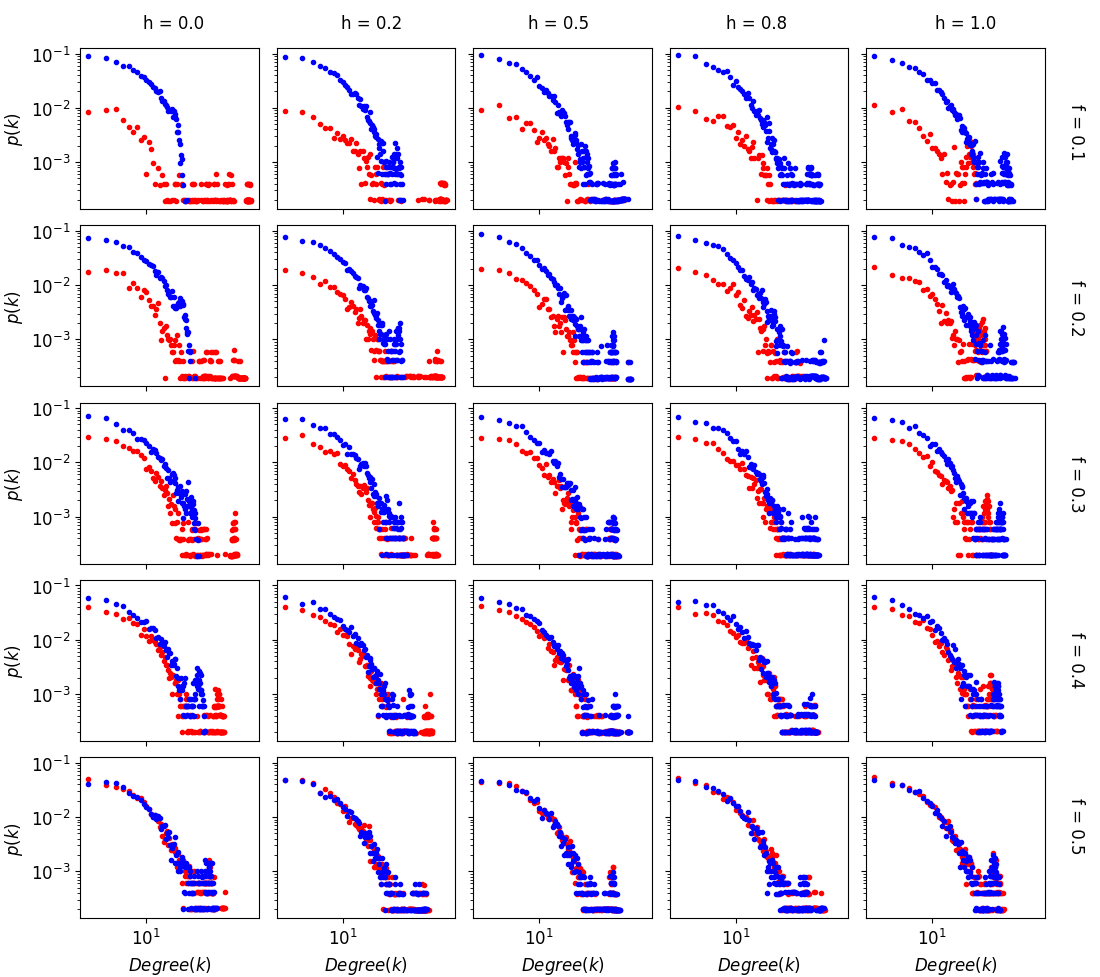
\includegraphics[width=1.0\textwidth]{images/dd_growth_top10.png}
	\caption{Degree distribution for growing networks with \textbf{Top-Rank ($r = 1.0$)}. The minority fractions are provided at the right-side of each row and the homophily values are specified at the top of each column. Degree distribution for the majority and minority nodes are visualized using blue and red plot points respectively.}
	\label{dd_growth_top10_fig}
\end{figure}

Upon looking at the degree growth plot (figure \ref{dg_growth_top10_fig}), we see that in the heterophilic regime the degree growth is much higher for minority nodes than majority nodes. This phenomenon has also been previously observed for synthetic networks which were influenced by the Karimi growth model. As we move towards the homophilic regime, the majority nodes gain higher degrees over minorities. We see a much faster degree growth for minorities than majority nodes in the heterophilic regime, and this can be attributed to the fact that the \textbf{Top-Rank} method is able to recommend minority nodes to majority with a much higher confidence (by having them at a greater precedence level). This confidence at placing nodes at higher precedence slots could also be the reason why at $f=0.1$ and $h=1$ we see that the minority nodes have higher degree growth than majority nodes.

\begin{figure}[h!]
	\centering
	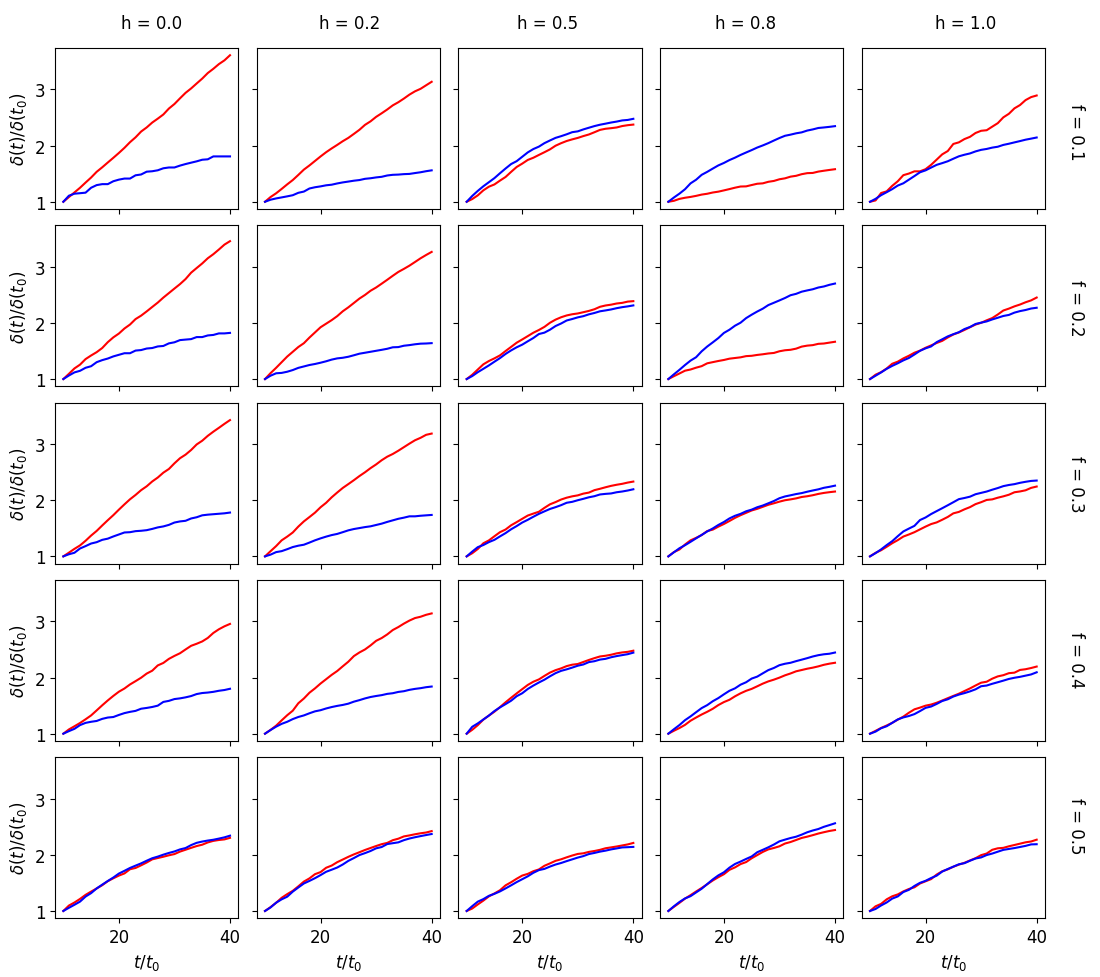
\includegraphics[width=1.0\textwidth]{images/dg_growth_top10.png}
	\caption{Degree growth for growing networks with \textbf{Top-Rank ($r = 1.0$)}. The minority fractions are provided at the right-side of each row and the homophily values are specified at the top of each column. Degree growth for minority and majority node is visualized using red and blue color plot lines respectively.}
	\label{dg_growth_top10_fig}
\end{figure}

Looking at the total degree held by minority nodes (figure \ref{mf_growth_top10_fig}) we also see similar results to what is expected. In the heterophilic regime, minority nodes hold higher degrees than their group-size, while in the homophilic regime they hold lower degrees which eventually is balanced out at complete homophily.

\begin{SCfigure}[1][h!]
	\centering
	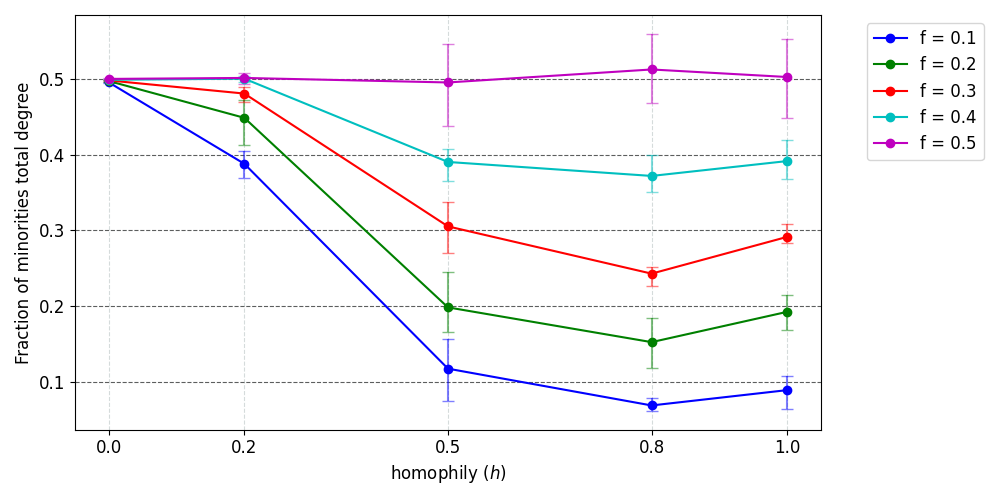
\includegraphics[trim=0 5 0 10, clip, width=0.75\textwidth]{images/mf_growth_top10.png}
	\caption{The fraction of total degree held by minority nodes for growing networks with \textbf{Top-Rank ($r = 1.0$)}.}
	\label{mf_growth_top10_fig}
\end{SCfigure}

The fraction of minorities in top D\% graph (figure \ref{top_growth_top10_fig}) show minorities being over-represented in the heterophilic regime, and underrepresented in the homophilic regime. This factor is also reduced as the minority group size increases. This shows the bias which is present in the click model is assimilated by the \textbf{Top-Rank} model as well, which causes the network to form in a similar fashion as the karimi model. 

\begin{figure}[h!]
	\centering
	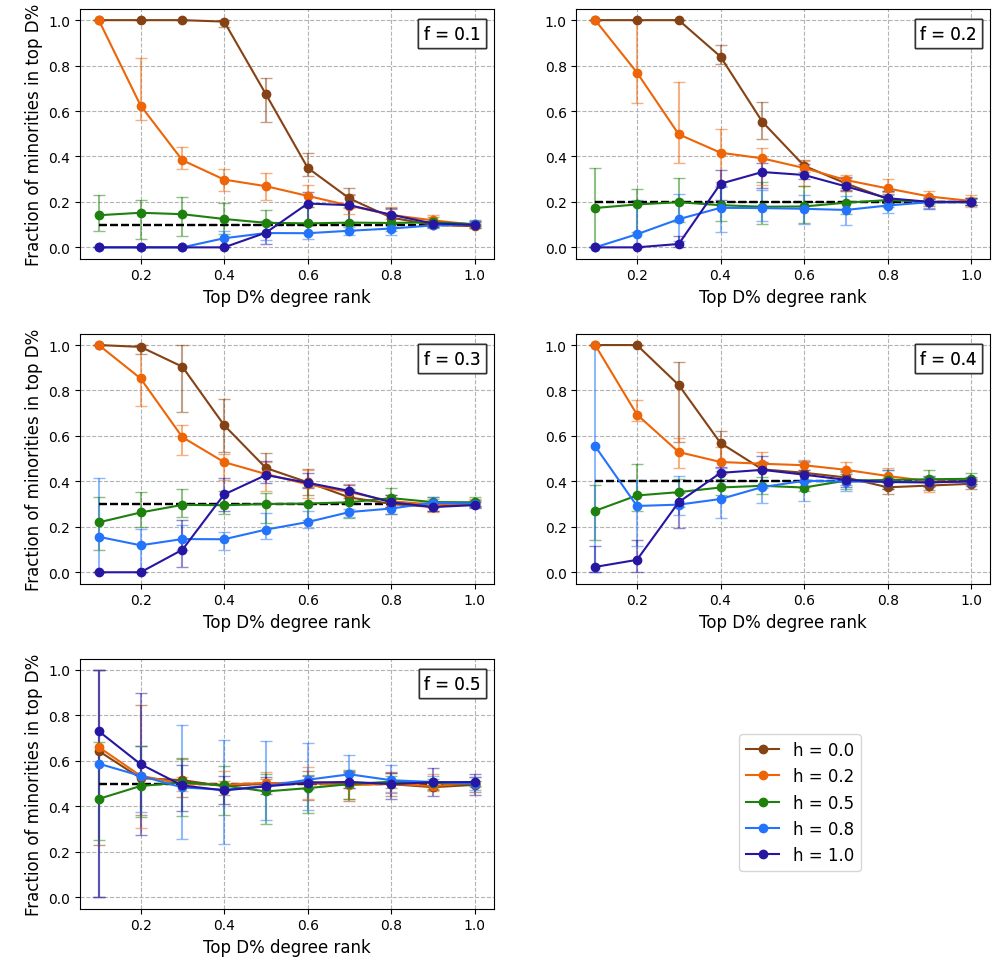
\includegraphics[trim=0 10 0 5, clip, width=1.0\textwidth]{images/top_growth_top10.png}
	\caption{The fraction of minority nodes found in top D\% nodes ranked according to degree in growing networks with \textbf{Top-Rank ($r = 1.0$)}. A black dotted line at each plot shows the actual fraction of minority nodes in the network.}
	\label{top_growth_top10_fig}
\end{figure}

\subsection{Summarized Findings}

We list down our major observations from the experiments on Growing Networks below.

\begin{enumerate}
	\item In \textbf{PA-Homophily} and the \textbf{reinforcement methods} we see similar plot patterns as observed for pre-generated static networks. This is due to the use of a \textit{click model} which is similar to the synthetic network generation method. It also shows that our reinforcement learning methods were able to correctly imbibe the traits of network and can be tuned internally to give better unbiased recommendations.
	
	\item The Randomness factor ($\mu$) in algorithm \ref{growing_network_model} causes the minorities to have over-representation in the complete homophily regime as there are connections established between nodes from opposite groups even in the case of complete homophily.
	
	\item \textbf{Adamic-Adar} is able to produce networks which are unbiased. This is possible at all cases of homophily other than in the strict heterophily case. Use of this recommendation method could lead to the evolution of a naturally balanced network with correct visibility for groups. Also it is observed that nodes tend to obtain really high degrees in this scenario.
	
	\item \textbf{Twitter-Rank} also provides us with correct representation of groups according to their groups sizes. The degree growth for networks using this recommendation mode is very slow owing to the use of personalized PageRank mechanism to form user's `circle of trust'. This makes node recommendations localized in nature.
\end{enumerate}